\documentclass[3p,times]{elsarticle}

\journal{Chinese Journal of Aeronautics}

\biboptions{sort&compress,super}   % CJA: references indicated by superscript numbers
\usepackage{amsmath,amssymb,amsfonts}
\usepackage{graphicx}
\usepackage{booktabs}
\usepackage{subcaption}
\usepackage{microtype}
\usepackage{xr-hyper}
\usepackage{hyperref}
\usepackage{url}
\usepackage{array}
\usepackage{multirow}
\usepackage{siunitx}
\sisetup{detect-all}

% Float placement optimization (prevents orphan float pages)
\renewcommand{\topfraction}{0.85}
\renewcommand{\bottomfraction}{0.85}
\renewcommand{\textfraction}{0.15}
\renewcommand{\floatpagefraction}{0.85}

\hypersetup{
    colorlinks=true,
    linkcolor=blue,
    citecolor=blue,
    urlcolor=blue
}

% generated by make_numbers.py; do not edit
\newcommand{\NeU}{203.3}
\newcommand{\NeUkJ}{732}
\newcommand{\NeF}{1.271}
\newcommand{\NpackNom}{864}
\newcommand{\NdbN}{10{,}087}
\newcommand{\NdbValid}{2{,}907}
\newcommand{\NpOneN}{9{,}800}
\newcommand{\NpOneValid}{2{,}750}
\newcommand{\NpOneValidPct}{28.1}
\newcommand{\NpTwoN}{287}
\newcommand{\NpTwoValid}{157}
\newcommand{\NpTwoValidPct}{55}
\newcommand{\NpOneBest}{352.9}
\newcommand{\NalOrigBest}{379.6}
\newcommand{\NalOrigUplift}{7.5}
\newcommand{\NchampRange}{379.6}
\newcommand{\NchampRangeRound}{380}
\newcommand{\NchLD}{17.12}
\newcommand{\NchCL}{0.247}
\newcommand{\NchSM}{0.225}
\newcommand{\NchCm}{-0.019}
\newcommand{\NchSref}{0.402}
\newcommand{\Nchmtot}{7.96}
\newcommand{\NchV}{36.67}
\newcommand{\Nchmbat}{3.40}
\newcommand{\NchCD}{0.0144}
\newcommand{\NchSMpct}{22.5}
\newcommand{\NchAR}{5.59}
\newcommand{\NchVkmh}{132}
\newcommand{\NacqN}{198}
\newcommand{\NuncN}{89}
\newcommand{\NacqValid}{91}
\newcommand{\NuncValid}{66}
\newcommand{\NnAL}{11}
\newcommand{\NnLoc}{10}
\newcommand{\NnAdapt}{10}
\newcommand{\NnALrep}{10}
\newcommand{\NnALstopped}{1}
\newcommand{\NalStopN}{117}
\newcommand{\NalStopBest}{371.1}
\newcommand{\NTurbomean}{396.6}
\newcommand{\NTurbosd}{5.8}
\newcommand{\NTurbolo}{385.1}
\newcommand{\NTurbohi}{403.0}
\newcommand{\NTurbon}{10}
\newcommand{\NTurbovr}{82}
\newcommand{\NTurbovrsixty}{80}
\newcommand{\NTurboupl}{12.4}
\newcommand{\NTurbofirstN}{10/10}
\newcommand{\NTurbofirstMed}{2}
\newcommand{\NALmean}{385.0}
\newcommand{\NALsd}{10.4}
\newcommand{\NALlo}{368.9}
\newcommand{\NALhi}{397.4}
\newcommand{\NALn}{11}
\newcommand{\NALvr}{59}
\newcommand{\NALvrsixty}{14}
\newcommand{\NALupl}{9.1}
\newcommand{\NALfirstN}{11/11}
\newcommand{\NALfirstMed}{43}
\newcommand{\NAdaptTenmean}{379.7}
\newcommand{\NAdaptTensd}{4.5}
\newcommand{\NAdaptTenlo}{370.8}
\newcommand{\NAdaptTenhi}{386.4}
\newcommand{\NAdaptTenn}{10}
\newcommand{\NAdaptTenvr}{71}
\newcommand{\NAdaptTenvrsixty}{72}
\newcommand{\NAdaptTenupl}{7.6}
\newcommand{\NAdaptTenfirstN}{10/10}
\newcommand{\NAdaptTenfirstMed}{51}
\newcommand{\NLocTenmean}{365.2}
\newcommand{\NLocTensd}{4.7}
\newcommand{\NLocTenlo}{358.5}
\newcommand{\NLocTenhi}{373.1}
\newcommand{\NLocTenn}{10}
\newcommand{\NLocTenvr}{64}
\newcommand{\NLocTenvrsixty}{60}
\newcommand{\NLocTenupl}{3.5}
\newcommand{\NLocTenfirstN}{10/10}
\newcommand{\NLocTenfirstMed}{36}
\newcommand{\NLocFivemean}{364.2}
\newcommand{\NLocFivesd}{6.6}
\newcommand{\NLocFivelo}{351.9}
\newcommand{\NLocFivehi}{373.2}
\newcommand{\NLocFiven}{10}
\newcommand{\NLocFivevr}{81}
\newcommand{\NLocFivevrsixty}{80}
\newcommand{\NLocFiveupl}{3.2}
\newcommand{\NLocFivefirstN}{9/10}
\newcommand{\NLocFivefirstMed}{31}
\newcommand{\NLhsmean}{298.3}
\newcommand{\NLhssd}{27.2}
\newcommand{\NLhslo}{260.2}
\newcommand{\NLhshi}{337.3}
\newcommand{\NLhsn}{10}
\newcommand{\NLhsvr}{28}
\newcommand{\NLhsvrsixty}{30}
\newcommand{\NLhsupl}{-15.5}
\newcommand{\NLhsfirstN}{0/10}
\newcommand{\NLhsfirstMed}{n/a}
\newcommand{\NUnimean}{307.6}
\newcommand{\NUnisd}{30.5}
\newcommand{\NUnilo}{264.2}
\newcommand{\NUnihi}{353.3}
\newcommand{\NUnin}{10}
\newcommand{\NUnivr}{28}
\newcommand{\NUnivrsixty}{26}
\newcommand{\NUniupl}{-12.9}
\newcommand{\NUnifirstN}{1/10}
\newcommand{\NUnifirstMed}{147}
\newcommand{\NdTurbo}{-11.6}
\newcommand{\NdTurbopct}{-2.9}
\newcommand{\NtTurbop}{0.005}
\newcommand{\NuTurbop}{0.007}
\newcommand{\NciTurbo}{[-18.4, -4.9]}
\newcommand{\NpsTurbo}{0.15}
\newcommand{\NdAdaptTen}{5.2}
\newcommand{\NdAdaptTenpct}{1.4}
\newcommand{\NtAdaptTenp}{0.150}
\newcommand{\NuAdaptTenp}{0.193}
\newcommand{\NciAdaptTen}{[-1.3, 11.6]}
\newcommand{\NpsAdaptTen}{0.67}
\newcommand{\NdLocTen}{19.8}
\newcommand{\NdLocTenpct}{5.4}
\newcommand{\NtLocTenp}{<0.001}
\newcommand{\NuLocTenp}{<0.001}
\newcommand{\NciLocTen}{[13.2, 26.1]}
\newcommand{\NpsLocTen}{0.96}
\newcommand{\NdLocFive}{20.7}
\newcommand{\NdLocFivepct}{5.7}
\newcommand{\NtLocFivep}{<0.001}
\newcommand{\NuLocFivep}{<0.001}
\newcommand{\NciLocFive}{[13.6, 27.7]}
\newcommand{\NpsLocFive}{0.96}
\newcommand{\NdLhs}{86.7}
\newcommand{\NdLhspct}{29.0}
\newcommand{\NtLhsp}{<0.001}
\newcommand{\NuLhsp}{<0.001}
\newcommand{\NciLhs}{[69.5, 103.5]}
\newcommand{\NpsLhs}{1.00}
\newcommand{\NdUni}{77.4}
\newcommand{\NdUnipct}{25.2}
\newcommand{\NtUnip}{<0.001}
\newcommand{\NuUnip}{<0.001}
\newcommand{\NciUni}{[58.1, 95.6]}
\newcommand{\NpsUni}{1.00}
\newcommand{\NdTurboAdapt}{16.9}
\newcommand{\NtTurboAdaptp}{<0.001}
\newcommand{\NciTurboAdapt}{[12.5, 21.1]}
\newcommand{\NciTurboOverAL}{[4.9, 18.4]}
\newcommand{\NdTurboOverAL}{11.6}
\newcommand{\NdTurboOverALpct}{3.0}
\newcommand{\NattrLocPct}{7.6}
\newcommand{\NattrShare}{84}
\newcommand{\NattrAlMeanPct}{9.1}
\newcommand{\NattrAlOverLocPct}{1.4}
\newcommand{\NattrOrigOverLocPct}{-0.0}
\newcommand{\NALexMean}{386.3}
\newcommand{\NALexN}{10}
\newcommand{\NatStopAL}{376.8}
\newcommand{\NatStopAdaptTen}{367.8}
\newcommand{\NatStopLocTen}{359.7}
\newcommand{\NatStopLocFive}{359.3}
\newcommand{\NstopAt}{117}
\newcommand{\NclampMean}{354.7}
\newcommand{\NnoclampMean}{350.0}
\newcommand{\NclampMinusPct}{1}
\newcommand{\NclampSeeds}{10}
\newcommand{\NclampP}{0.83}
\newcommand{\NclampValid}{55}
\newcommand{\NnoclampValid}{47}
\newcommand{\NinvShare}{7}
\newcommand{\NpaperBndMean}{361.3}
\newcommand{\NwideBndMean}{432.6}
\newcommand{\NwideGainPct}{20}
\newcommand{\NclampActWide}{3}
\newcommand{\NwideBndMax}{474}
\newcommand{\NAbN}{1000}
\newcommand{\NAbNinv}{355}
\newcommand{\NAbVinv}{137}
\newcommand{\NAbVmono}{212}
\newcommand{\NAbVRinv}{39}
\newcommand{\NAbVRmono}{33}
\newcommand{\NAbLDinv}{7.65}
\newcommand{\NAbLDmono}{9.82}
\newcommand{\NAbMedInv}{7.37}
\newcommand{\NAbMedMono}{9.37}
\newcommand{\NAbSinv}{0.69}
\newcommand{\NAbSmono}{0.46}
\newcommand{\NAbARinv}{3.27}
\newcommand{\NAbARmono}{5.17}
\newcommand{\NAbRho}{-0.48}
\newcommand{\NAbMatchN}{40+65}
\newcommand{\NAbMatchInv}{8.13}
\newcommand{\NAbMatchMono}{8.41}
\newcommand{\NAbMatchP}{0.49}
\newcommand{\NAbOLS}{0.63}
\newcommand{\NAbOLSse}{0.18}
\newcommand{\NAbSlo}{0.53}
\newcommand{\NAbShi}{0.67}
\newcommand{\NAbMaxRinv}{268}
\newcommand{\NAbMaxRmono}{393}
\newcommand{\NmonoN}{2{,}907}
\newcommand{\NmonoShare}{22\%}
\newcommand{\NmonoMed}{1.6}
\newcommand{\NmonoMax}{5.3}
\newcommand{\NmonoGone}{15\% of all valid designs}
\newcommand{\NfnRecall}{58.5}
\newcommand{\NfnRecallSd}{2.3}
\newcommand{\NfnPrec}{88.5}
\newcommand{\NfnPrecSd}{2.0}
\newcommand{\NfnTenRecall}{77.2}
\newcommand{\NfnTenRecallSd}{3.8}
\newcommand{\NfnTwoRecall}{89.3}
\newcommand{\NfnTwoRecallSd}{2.9}
\newcommand{\NfnMeanP}{0.686}
\newcommand{\NfnMeanPSd}{0.015}
\newcommand{\NfnTenN}{54--60}
\newcommand{\NfnTwoN}{9--17}
\newcommand{\NfnTestValid}{582}
\newcommand{\NfnWithin}{26}
\newcommand{\NtpWithin}{9}
\newcommand{\NfnMedian}{121}
\newcommand{\NtpMedian}{135}
\newcommand{\NfnMax}{375}
\newcommand{\NfnMaxSplit}{380}
\newcommand{\NclfInfeasShare}{71.2}
\newcommand{\NclfNrows}{10{,}087}
\newcommand{\NclfNvalid}{2{,}907}
\newcommand{\NpoolInfeasShare}{71.9}
\newcommand{\NpoolValidN}{2{,}750}
\newcommand{\NclfQten}{249.4}
\newcommand{\NclfQtwo}{371.8}
\newcommand{\NclfQtenRaw}{196.3}
\newcommand{\NclfQtwoRaw}{292.6}
\newcommand{\NfnRecallUnscaled}{54.3}
\newcommand{\NfnPrecUnscaled}{89.7}
\newcommand{\NcvRange}{0.997}
\newcommand{\NcvRangeMape}{2.3}
\newcommand{\NshiftRtwo}{0.76}
\newcommand{\NshiftMae}{3.7}
\newcommand{\NshiftBias}{3.7}
\newcommand{\NshiftTopRho}{-0.05}
\newcommand{\NextrapRtwo}{0.35}
\newcommand{\NextrapBias}{8.3}
\newcommand{\NextrapCover}{0.59}
\newcommand{\NshiftCover}{0.78}
\newcommand{\NxN}{72}
\newcommand{\NxRho}{0.98}
\newcommand{\NxRhoTop}{0.91}
\newcommand{\NxRhoRand}{0.99}
\newcommand{\NxRatioMed}{1.46}
\newcommand{\NxRatioLo}{1.35}
\newcommand{\NxRatioHi}{1.77}
\newcommand{\NxNtop}{36}
\newcommand{\NgridTopLD}{1.5}
\newcommand{\NgridSM}{0.009}
\newcommand{\NgridTopCL}{0.02}
\newcommand{\NgridMedLD}{10}
\newcommand{\NgridPtenLD}{20}
\newcommand{\NgridPtenLDx}{2}
\newcommand{\NgridMedLDx}{7}
\newcommand{\NgridMaxPanels}{3{,}584}
\newcommand{\NcfdN}{5}
\newcommand{\NcfdSMlo}{1.14}
\newcommand{\NcfdSMhi}{1.28}
\newcommand{\NcfdCLlo}{0.97}
\newcommand{\NcfdCLhi}{1.04}
\newcommand{\NcfdSlope}{0.064}
\newcommand{\NcfdChampSM}{0.258}
\newcommand{\NcfdChampSMratio}{1.14}
\newcommand{\NcfdChampCL}{1.04}
\newcommand{\NcfdChampHave}{1}
\newcommand{\NnfLo}{0.60}
\newcommand{\NnfHi}{0.67}
\newcommand{\NnfTurbRatio}{1.18}
\newcommand{\NnfChampLDgain}{1.33}
\newcommand{\NbBsource}{al\_seed0.csv:271}
\newcommand{\NbARange}{379.6}
\newcommand{\NbARangeSnap}{379.4}
\newcommand{\NbARangeSnapRound}{379}
\newcommand{\NbALD}{17.12}
\newcommand{\NbACL}{0.247}
\newcommand{\NbASM}{0.225}
\newcommand{\NbACm}{-0.019}
\newcommand{\NbASref}{0.402}
\newcommand{\NbAAR}{5.59}
\newcommand{\NbAmtot}{7.96}
\newcommand{\NbAVkmh}{132}
\newcommand{\NbAmb}{3.40}
\newcommand{\NbASMsnap}{0.225}
\newcommand{\NbATrim}{1.1}
\newcommand{\NbBRange}{394.4}
\newcommand{\NbBRangeSnap}{385.2}
\newcommand{\NbBRangeSnapRound}{385}
\newcommand{\NbBLD}{17.50}
\newcommand{\NbBCL}{0.256}
\newcommand{\NbBSM}{0.183}
\newcommand{\NbBCm}{-0.013}
\newcommand{\NbBSref}{0.396}
\newcommand{\NbBAR}{5.68}
\newcommand{\NbBmtot}{8.04}
\newcommand{\NbBVkmh}{131}
\newcommand{\NbBmb}{3.50}
\newcommand{\NbBSMsnap}{0.187}
\newcommand{\NbBTrim}{0.5}
\newcommand{\NbSnapLossPct}{2.3}
\newcommand{\NbBoverAPct}{1.5}
\newcommand{\NbASMeuler}{0.258}
\newcommand{\NbACLratio}{1.04}
\newcommand{\NbBSMeuler}{0.221}
\newcommand{\NbBCLratio}{0.97}
\newcommand{\NmassALo}{+3}
\newcommand{\NmassALoRange}{390}
\newcommand{\NmassAHi}{-3}
\newcommand{\NmassAHiRange}{368}
\newcommand{\NbayAGain}{1.1}
\newcommand{\NbayASMlo}{0.11}
\newcommand{\NbayASMbase}{0.225}
\newcommand{\NbayAFwdLimit}{0.82}
\newcommand{\NmassBLo}{+3}
\newcommand{\NmassBLoRange}{405}
\newcommand{\NmassBHi}{-3}
\newcommand{\NmassBHiRange}{384}
\newcommand{\NbayBGain}{0.5}
\newcommand{\NbayBSMlo}{0.07}
\newcommand{\NbayBSMbase}{0.183}
\newcommand{\NbayBFwdLimit}{0.74}
\newcommand{\NtopTaperLo}{60}
\newcommand{\NtopWtHi}{100}
\newcommand{\NtopVLo}{85}
\newcommand{\NchAtBound}{4}
\newcommand{\NtopAtBoundN}{3}
\newcommand{\NvolProxy}{2.88}
\newcommand{\NvolLoft}{3.11}
\newcommand{\NvolDiff}{8\%}
\newcommand{\NcellVol}{1.25}
\newcommand{\NclampActPaper}{0}
\newcommand{\NchTrimDrag}{1.1}
\newcommand{\NeuLo}{195}
\newcommand{\NeuHi}{216}
\newcommand{\NeuLoPct}{4}
\newcommand{\NeuHiPct}{6}
\newcommand{\NcellKg}{3.312}
\newcommand{\NoverheadG}{88}
\newcommand{\NsmLimLo}{0.22}
\newcommand{\NsmDbLo}{377}
\newcommand{\NsmAllLo}{397}
\newcommand{\NsmExclLo}{14}
\newcommand{\NsmLimMid}{0.21}
\newcommand{\NsmDbMid}{377}
\newcommand{\NsmAllMid}{397}
\newcommand{\NsmExclMid}{22}
\newcommand{\NsmLimHi}{0.20}
\newcommand{\NsmDbHi}{377}
\newcommand{\NsmAllHi}{397}
\newcommand{\NsmExclHi}{29}
\newcommand{\NsmAllNone}{397}
\newcommand{\NalSMlo}{0.12}
\newcommand{\NalSMhi}{0.23}
\newcommand{\NbAlSoftMean}{385.5}
\newcommand{\NbAlSoftSd}{10.8}
\newcommand{\NbAlSoftN}{10}
\newcommand{\NbAlSoftValid}{60}
\newcommand{\NbAlSoftVSixty}{14}
\newcommand{\NbAlSoftMin}{368.9}
\newcommand{\NbAlSoftMax}{397.4}
\newcommand{\NbAlHardMean}{394.0}
\newcommand{\NbAlHardSd}{4.2}
\newcommand{\NbAlHardN}{10}
\newcommand{\NbAlHardValid}{10}
\newcommand{\NbAlHardVSixty}{0}
\newcommand{\NbAlHardMin}{383.6}
\newcommand{\NbAlHardMax}{399.5}
\newcommand{\NbTurboMean}{396.6}
\newcommand{\NbTurboSd}{5.8}
\newcommand{\NbTurboN}{10}
\newcommand{\NbTurboValid}{82}
\newcommand{\NbTurboVSixty}{80}
\newcommand{\NbTurboMin}{385.1}
\newcommand{\NbTurboMax}{403.0}
\newcommand{\NbTurboFeasMean}{394.8}
\newcommand{\NbTurboFeasSd}{4.4}
\newcommand{\NbTurboFeasN}{10}
\newcommand{\NbTurboFeasValid}{91}
\newcommand{\NbTurboFeasVSixty}{90}
\newcommand{\NbTurboFeasMin}{386.2}
\newcommand{\NbTurboFeasMax}{399.5}
\newcommand{\NbAlNoneN}{10}
\newcommand{\NbAlNoneValid}{0}
\newcommand{\NbAlHardAtHundred}{0.0}
\newcommand{\NbAlHardAtOneFifty}{38.4}
\newcommand{\NbAlHardOverSoftD}{8.5}
\newcommand{\NbAlHardOverSoftWelch}{0.039}
\newcommand{\NbAlHardOverSoftMwu}{0.076}
\newcommand{\NbAlHardOverSoftCI}{[1.9, 15.4]}
\newcommand{\NbTurboFeasOverTurboD}{-1.8}
\newcommand{\NbTurboFeasOverTurboWelch}{0.437}
\newcommand{\NbTurboFeasOverTurboMwu}{0.212}
\newcommand{\NbTurboFeasOverTurboCI}{[-6.0, 2.5]}
\newcommand{\NbTurboOverAlRepD}{11.1}
\newcommand{\NbTurboOverAlRepWelch}{0.012}
\newcommand{\NbTurboOverAlRepMwu}{0.011}
\newcommand{\NbTurboOverAlRepCI}{[4.1, 18.5]}
\newcommand{\NbTurboFeasOverAlRepD}{9.3}
\newcommand{\NbTurboFeasOverAlRepWelch}{0.027}
\newcommand{\NbTurboFeasOverAlRepMwu}{0.021}
\newcommand{\NbTurboFeasOverAlRepCI}{[2.6, 16.3]}
\newcommand{\NbAlRepOverAdaptD}{5.8}
\newcommand{\NbAlRepOverAdaptWelch}{0.143}
\newcommand{\NbAlRepOverAdaptMwu}{0.121}
\newcommand{\NbAlRepOverAdaptCI}{[-1.2, 12.4]}
\newcommand{\NbAlRepOverLocTenD}{20.3}
\newcommand{\NbAlRepOverLocTenWelch}{<0.001}
\newcommand{\NbAlRepOverLocTenMwu}{<0.001}
\newcommand{\NbAlRepOverLocTenCI}{[13.3, 26.9]}
\newcommand{\NbTurboOverAdaptD}{16.9}
\newcommand{\NbTurboOverAdaptWelch}{<0.001}
\newcommand{\NbTurboOverAdaptMwu}{<0.001}
\newcommand{\NbTurboOverAdaptCI}{[12.5, 21.1]}
\newcommand{\NbAdaptMean}{379.7}
\newcommand{\NbAdaptN}{10}
\newcommand{\NbLocTenMean}{365.2}
\newcommand{\NbLocTenN}{10}
\newcommand{\NbLocFiveMean}{364.2}
\newcommand{\NbLocFiveN}{10}
\newcommand{\NbLhsMean}{298.3}
\newcommand{\NbLhsN}{10}
\newcommand{\NbUniMean}{307.6}
\newcommand{\NbUniN}{10}
\newcommand{\NcalN}{20}
\newcommand{\NcalA}{0.035}
\newcommand{\NcalB}{0.984}
\newcommand{\NcalAci}{[0.032, 0.041]}
\newcommand{\NcalBci}{[0.958, 1.003]}
\newcommand{\NcalRsq}{0.997}
\newcommand{\NcalSd}{0.003}
\newcommand{\NcalCapEquiv}{0.218}
\newcommand{\NcalFloorEquiv}{0.015}
\newcommand{\NcalCLmed}{1.009}
\newcommand{\NcalCLlo}{0.967}
\newcommand{\NcalCLhi}{1.193}
\newcommand{\NcalOffsetMean}{0.033}
\newcommand{\NcalOffsetMin}{0.027}
\newcommand{\NcalOffsetMax}{0.040}
\newcommand{\NcalNnew}{15}
\newcommand{\NcalAlHfiveSM}{0.223}
\newcommand{\NcalAlHsevenSM}{0.227}
\newcommand{\NcalAlHdelta}{-1.5}
\newcommand{\NcalAlHfiveNodes}{203}
\newcommand{\NcalAlHfiveCL}{0.262}
\newcommand{\NcalAlHsevenCL}{0.263}
\newcommand{\NcalOutAlSoft}{0}
\newcommand{\NcalOutNAlSoft}{10}
\newcommand{\NcalLossAlSoft}{0.0}
\newcommand{\NcalOutAlR}{4}
\newcommand{\NcalOutNAlR}{20}
\newcommand{\NcalLossAlR}{0.2}
\newcommand{\NcalOutTurbo}{1}
\newcommand{\NcalOutNTurbo}{20}
\newcommand{\NcalLossTurbo}{0.0}
\newcommand{\NcalOutTurboFeas}{0}
\newcommand{\NcalOutNTurboFeas}{10}
\newcommand{\NcalLossTurboFeas}{0.0}
\newcommand{\NcalOutAlHard}{3}
\newcommand{\NcalOutNAlHard}{10}
\newcommand{\NcalLossAlHard}{0.9}
\newcommand{\NcalOutAdapt}{3}
\newcommand{\NcalOutNAdapt}{20}
\newcommand{\NcalLossAdapt}{0.2}
\newcommand{\NcalOutLocTen}{4}
\newcommand{\NcalOutNLocTen}{10}
\newcommand{\NcalLossLocTen}{3.1}
\newcommand{\NcalOutLocFive}{1}
\newcommand{\NcalOutNLocFive}{10}
\newcommand{\NcalLossLocFive}{0.3}
\newcommand{\NcalOutLhs}{2}
\newcommand{\NcalOutNLhs}{10}
\newcommand{\NcalLossLhs}{7.3}
\newcommand{\NcalOutUni}{2}
\newcommand{\NcalOutNUni}{10}
\newcommand{\NcalLossUni}{1.6}
\newcommand{\NcalLossArmMax}{7.3}
\newcommand{\NbpBmassMassPct}{5.7}
\newcommand{\NbpRefMean}{396.3}
\newcommand{\NbpRefSd}{5.3}
\newcommand{\NbpTaperN}{5}
\newcommand{\NbpTaperMean}{398.7}
\newcommand{\NbpTaperGain}{2.4}
\newcommand{\NbpTaperGainPct}{0.6}
\newcommand{\NbpTaperCI}{[-4.5, 8.3]}
\newcommand{\NbpTaperP}{0.530}
\newcommand{\NbpTaperAtBound}{60}
\newcommand{\NbpWtwistN}{5}
\newcommand{\NbpWtwistMean}{395.7}
\newcommand{\NbpWtwistGain}{-0.6}
\newcommand{\NbpWtwistGainPct}{-0.1}
\newcommand{\NbpWtwistCI}{[-5.1, 4.0]}
\newcommand{\NbpWtwistP}{0.831}
\newcommand{\NbpWtwistAtBound}{0}
\newcommand{\NbpBmassN}{5}
\newcommand{\NbpBmassMean}{417.3}
\newcommand{\NbpBmassGain}{21.0}
\newcommand{\NbpBmassGainPct}{5.3}
\newcommand{\NbpBmassCI}{[17.2, 25.0]}
\newcommand{\NbpBmassP}{<0.001}
\newcommand{\NbpBmassAtBound}{100}
\newcommand{\NbpSpeedN}{5}
\newcommand{\NbpSpeedMean}{395.8}
\newcommand{\NbpSpeedGain}{-0.5}
\newcommand{\NbpSpeedGainPct}{-0.1}
\newcommand{\NbpSpeedCI}{[-4.5, 3.9]}
\newcommand{\NbpSpeedP}{0.831}
\newcommand{\NbpSpeedAtBound}{0}
\newcommand{\NrbN}{27}
\newcommand{\NrbAllValid}{12}
\newcommand{\NrbBandValid}{24}
\newcommand{\NrbPfiveInvalid}{13}
\newcommand{\NrbOswald}{13}
\newcommand{\NrbAllBest}{top02}
\newcommand{\NrbAllBestRange}{402.4}
\newcommand{\NrbAllBestBandLoss}{0.4}
\newcommand{\NrbAllBestMfiveLoss}{4.1}
\newcommand{\NrbAllBestPfiveGain}{4.0}
\newcommand{\NrbBandBest}{top01}
\newcommand{\NrbBandBestRange}{403.0}
\newcommand{\NrbBandBestLoss}{0.5}
\newcommand{\NrbBandLossMax}{0.8}
\newcommand{\NrbMfiveLossMean}{4.2}

\newcommand{\NADAPTCONC}{An adaptive surrogate-free local search, which re-seeds around the best designs found so far, reaches \NAdaptTenmean\,km and is within \NdAdaptTen\,km of active learning (interval \NciAdaptTen\,km, including zero); the experiment therefore does not show a contribution of the surrogate beyond adaptive local refinement.}
\newcommand{\NADAPTABS}{An adaptive surrogate-free local search that re-seeds around the best designs reaches \NAdaptTenmean\,km, within \NdAdaptTenpct\,\% of active learning (interval includes zero), so a contribution of the surrogate itself is not demonstrated.}
\newcommand{\NADAPTRESP}{We added the control that isolates the surrogate: an adaptive local search with the same cycle structure and seed rule as the loop but no model (Sec.~5.1, Table~6). It reaches \NAdaptTenmean\,km over \NAdaptTenn\ runs, against \NALmean\,km for active learning; the difference is \NdAdaptTen\,km (\NdAdaptTenpct\,\%) with a bootstrap interval \NciAdaptTen\,km that includes zero. We therefore state plainly that the +7.5\,\% cannot be attributed to the surrogate and that this study does not show a surrogate benefit over adaptive local search.}

% generated by make_numbers_v4.py; do not edit
\newcommand{\NvNTurbo}{20}
\newcommand{\NvMeanTurbo}{396.8}
\newcommand{\NvSdTurbo}{4.4}
\newcommand{\NvMinTurbo}{385.3}
\newcommand{\NvMaxTurbo}{403.0}
\newcommand{\NvValidTurbo}{82}
\newcommand{\NvFirstTurbo}{80}
\newcommand{\NvWashTurbo}{0}
\newcommand{\NvGainTurbo}{43.8}
\newcommand{\NvGainPctTurbo}{12.4}
\newcommand{\NvAtHundTurbo}{382.9}
\newcommand{\NvNALR}{20}
\newcommand{\NvMeanALR}{391.5}
\newcommand{\NvSdALR}{6.6}
\newcommand{\NvMinALR}{367.9}
\newcommand{\NvMaxALR}{399.5}
\newcommand{\NvValidALR}{64}
\newcommand{\NvFirstALR}{24}
\newcommand{\NvWashALR}{0}
\newcommand{\NvGainALR}{38.5}
\newcommand{\NvGainPctALR}{10.9}
\newcommand{\NvAtHundALR}{378.8}
\newcommand{\NvNAL}{11}
\newcommand{\NvMeanAL}{385.0}
\newcommand{\NvSdAL}{10.4}
\newcommand{\NvMinAL}{368.9}
\newcommand{\NvMaxAL}{397.4}
\newcommand{\NvValidAL}{59}
\newcommand{\NvFirstAL}{14}
\newcommand{\NvWashAL}{17}
\newcommand{\NvGainAL}{32.0}
\newcommand{\NvGainPctAL}{9.1}
\newcommand{\NvAtHundAL}{374.1}
\newcommand{\NvNAdapt}{20}
\newcommand{\NvMeanAdapt}{386.1}
\newcommand{\NvSdAdapt}{6.3}
\newcommand{\NvMinAdapt}{369.2}
\newcommand{\NvMaxAdapt}{393.2}
\newcommand{\NvValidAdapt}{68}
\newcommand{\NvFirstAdapt}{69}
\newcommand{\NvWashAdapt}{0}
\newcommand{\NvGainAdapt}{33.1}
\newcommand{\NvGainPctAdapt}{9.4}
\newcommand{\NvAtHundAdapt}{372.9}
\newcommand{\NvNLocTen}{10}
\newcommand{\NvMeanLocTen}{365.2}
\newcommand{\NvSdLocTen}{4.7}
\newcommand{\NvMinLocTen}{358.5}
\newcommand{\NvMaxLocTen}{373.1}
\newcommand{\NvValidLocTen}{64}
\newcommand{\NvFirstLocTen}{60}
\newcommand{\NvWashLocTen}{0}
\newcommand{\NvGainLocTen}{12.2}
\newcommand{\NvGainPctLocTen}{3.5}
\newcommand{\NvAtHundLocTen}{358.8}
\newcommand{\NvNLocFive}{10}
\newcommand{\NvMeanLocFive}{364.2}
\newcommand{\NvSdLocFive}{6.6}
\newcommand{\NvMinLocFive}{351.9}
\newcommand{\NvMaxLocFive}{373.2}
\newcommand{\NvValidLocFive}{81}
\newcommand{\NvFirstLocFive}{80}
\newcommand{\NvWashLocFive}{0}
\newcommand{\NvGainLocFive}{11.3}
\newcommand{\NvGainPctLocFive}{3.2}
\newcommand{\NvAtHundLocFive}{359.3}
\newcommand{\NvNLhs}{10}
\newcommand{\NvMeanLhs}{298.3}
\newcommand{\NvSdLhs}{27.2}
\newcommand{\NvMinLhs}{260.2}
\newcommand{\NvMaxLhs}{337.3}
\newcommand{\NvValidLhs}{28}
\newcommand{\NvFirstLhs}{30}
\newcommand{\NvWashLhs}{0}
\newcommand{\NvGainLhs}{-54.6}
\newcommand{\NvGainPctLhs}{-15.5}
\newcommand{\NvAtHundLhs}{352.9}
\newcommand{\NvNUni}{10}
\newcommand{\NvMeanUni}{307.6}
\newcommand{\NvSdUni}{30.5}
\newcommand{\NvMinUni}{264.2}
\newcommand{\NvMaxUni}{353.3}
\newcommand{\NvValidUni}{28}
\newcommand{\NvFirstUni}{26}
\newcommand{\NvWashUni}{0}
\newcommand{\NvGainUni}{-45.4}
\newcommand{\NvGainPctUni}{-12.9}
\newcommand{\NvAtHundUni}{352.9}
\newcommand{\NvNALRc}{19}
\newcommand{\NvMeanALRc}{392.7}
\newcommand{\NvSdALRc}{3.6}
\newcommand{\NvMinALRc}{385.4}
\newcommand{\NvMaxALRc}{399.5}
\newcommand{\NvValidALRc}{66}
\newcommand{\NvFirstALRc}{25}
\newcommand{\NvWashALRc}{0}
\newcommand{\NvGainALRc}{39.8}
\newcommand{\NvGainPctALRc}{11.3}
\newcommand{\NvAtHundALRc}{379.4}
\newcommand{\NvNTurboOld}{10}
\newcommand{\NvMeanTurboOld}{396.6}
\newcommand{\NvSdTurboOld}{5.8}
\newcommand{\NvMinTurboOld}{385.1}
\newcommand{\NvMaxTurboOld}{403.0}
\newcommand{\NvValidTurboOld}{82}
\newcommand{\NvFirstTurboOld}{80}
\newcommand{\NvWashTurboOld}{0}
\newcommand{\NvGainTurboOld}{43.7}
\newcommand{\NvGainPctTurboOld}{12.4}
\newcommand{\NvAtHundTurboOld}{381.0}
\newcommand{\NvNAdaptOld}{10}
\newcommand{\NvMeanAdaptOld}{379.7}
\newcommand{\NvSdAdaptOld}{4.5}
\newcommand{\NvMinAdaptOld}{370.8}
\newcommand{\NvMaxAdaptOld}{386.4}
\newcommand{\NvValidAdaptOld}{71}
\newcommand{\NvFirstAdaptOld}{72}
\newcommand{\NvWashAdaptOld}{0}
\newcommand{\NvGainAdaptOld}{26.8}
\newcommand{\NvGainPctAdaptOld}{7.6}
\newcommand{\NvAtHundAdaptOld}{365.4}
\newcommand{\NvNALrep}{10}
\newcommand{\NvMeanALrep}{385.5}
\newcommand{\NvSdALrep}{10.8}
\newcommand{\NvMinALrep}{368.9}
\newcommand{\NvMaxALrep}{397.4}
\newcommand{\NvValidALrep}{60}
\newcommand{\NvFirstALrep}{14}
\newcommand{\NvWashALrep}{17}
\newcommand{\NvGainALrep}{32.6}
\newcommand{\NvGainPctALrep}{9.2}
\newcommand{\NvAtHundALrep}{376.1}
\newcommand{\NvNALhard}{10}
\newcommand{\NvMeanALhard}{394.0}
\newcommand{\NvSdALhard}{4.2}
\newcommand{\NvMinALhard}{383.6}
\newcommand{\NvMaxALhard}{399.5}
\newcommand{\NvValidALhard}{10}
\newcommand{\NvFirstALhard}{0}
\newcommand{\NvWashALhard}{64}
\newcommand{\NvGainALhard}{41.0}
\newcommand{\NvGainPctALhard}{11.6}
\newcommand{\NvAtHundALhard}{352.9}
\newcommand{\NvNALnone}{10}
\newcommand{\NvValidALnone}{0}
\newcommand{\NvWashALnone}{100}
\newcommand{\NvNALRnone}{10}
\newcommand{\NvValidALRnone}{0}
\newcommand{\NvWashALRnone}{0}
\newcommand{\NvNALRten}{10}
\newcommand{\NvMeanALRten}{394.0}
\newcommand{\NvSdALRten}{4.1}
\newcommand{\NvMinALRten}{386.3}
\newcommand{\NvMaxALRten}{399.5}
\newcommand{\NvValidALRten}{65}
\newcommand{\NvFirstALRten}{26}
\newcommand{\NvWashALRten}{0}
\newcommand{\NvGainALRten}{41.1}
\newcommand{\NvGainPctALRten}{11.6}
\newcommand{\NvAtHundALRten}{379.8}
\newcommand{\NvNTurboFeasFix}{10}
\newcommand{\NvMeanTurboFeasFix}{397.5}
\newcommand{\NvSdTurboFeasFix}{2.8}
\newcommand{\NvMinTurboFeasFix}{394.0}
\newcommand{\NvMaxTurboFeasFix}{403.0}
\newcommand{\NvValidTurboFeasFix}{92}
\newcommand{\NvFirstTurboFeasFix}{92}
\newcommand{\NvWashTurboFeasFix}{0}
\newcommand{\NvGainTurboFeasFix}{44.6}
\newcommand{\NvGainPctTurboFeasFix}{12.6}
\newcommand{\NvAtHundTurboFeasFix}{383.9}
\newcommand{\NvNTurboFeas}{10}
\newcommand{\NvMeanTurboFeas}{394.8}
\newcommand{\NvSdTurboFeas}{4.4}
\newcommand{\NvMinTurboFeas}{386.2}
\newcommand{\NvMaxTurboFeas}{399.5}
\newcommand{\NvValidTurboFeas}{91}
\newcommand{\NvFirstTurboFeas}{90}
\newcommand{\NvWashTurboFeas}{0}
\newcommand{\NvGainTurboFeas}{41.8}
\newcommand{\NvGainPctTurboFeas}{11.8}
\newcommand{\NvAtHundTurboFeas}{376.8}
\newcommand{\NvDTurbovALR}{5.3}
\newcommand{\NvDsTurbovALR}{+5.3}
\newcommand{\NvPctTurbovALR}{1.4}
\newcommand{\NvPTurbovALR}{= 0.005}
\newcommand{\NvUTurbovALR}{= 0.001}
\newcommand{\NvCITurbovALR}{[2.2, 8.8]}
\newcommand{\NvHiTurbovALR}{8.8}
\newcommand{\NvHiPctTurbovALR}{2.3}
\newcommand{\NvHTurbovALR}{= 0.020}
\newcommand{\NvDALRvAL}{6.5}
\newcommand{\NvDsALRvAL}{+6.5}
\newcommand{\NvPctALRvAL}{1.7}
\newcommand{\NvPALRvAL}{= 0.079}
\newcommand{\NvUALRvAL}{= 0.180}
\newcommand{\NvCIALRvAL}{[0.1, 12.9]}
\newcommand{\NvHiALRvAL}{12.9}
\newcommand{\NvHiPctALRvAL}{3.4}
\newcommand{\NvHALRvAL}{= 0.159}
\newcommand{\NvDALRvAdapt}{5.4}
\newcommand{\NvDsALRvAdapt}{+5.4}
\newcommand{\NvPctALRvAdapt}{1.4}
\newcommand{\NvPALRvAdapt}{= 0.011}
\newcommand{\NvUALRvAdapt}{= 0.003}
\newcommand{\NvCIALRvAdapt}{[1.4, 9.2]}
\newcommand{\NvHiALRvAdapt}{9.2}
\newcommand{\NvHiPctALRvAdapt}{2.4}
\newcommand{\NvHALRvAdapt}{= 0.033}
\newcommand{\NvDTurbovAdapt}{10.7}
\newcommand{\NvDsTurbovAdapt}{+10.7}
\newcommand{\NvPctTurbovAdapt}{2.8}
\newcommand{\NvPTurbovAdapt}{< 0.001}
\newcommand{\NvUTurbovAdapt}{< 0.001}
\newcommand{\NvCITurbovAdapt}{[7.5, 14.1]}
\newcommand{\NvHiTurbovAdapt}{14.1}
\newcommand{\NvHiPctTurbovAdapt}{3.6}
\newcommand{\NvHTurbovAdapt}{< 0.001}
\newcommand{\NvDALvAdapt}{1.1}
\newcommand{\NvDsALvAdapt}{-1.1}
\newcommand{\NvPctALvAdapt}{0.3}
\newcommand{\NvPALvAdapt}{= 0.752}
\newcommand{\NvUALvAdapt}{= 0.918}
\newcommand{\NvCIALvAdapt}{[-7.6, 5.1]}
\newcommand{\NvHiALvAdapt}{7.6}
\newcommand{\NvHiPctALvAdapt}{2.0}
\newcommand{\NvHALvAdapt}{= 0.752}
\newcommand{\NvDAdaptvLocTen}{20.9}
\newcommand{\NvDsAdaptvLocTen}{+20.9}
\newcommand{\NvPctAdaptvLocTen}{5.7}
\newcommand{\NvPAdaptvLocTen}{< 0.001}
\newcommand{\NvUAdaptvLocTen}{< 0.001}
\newcommand{\NvCIAdaptvLocTen}{[16.9, 24.6]}
\newcommand{\NvHiAdaptvLocTen}{24.6}
\newcommand{\NvHiPctAdaptvLocTen}{6.7}
\newcommand{\NvHAdaptvLocTen}{< 0.001}
\newcommand{\NvDALvLocTen}{19.8}
\newcommand{\NvDsALvLocTen}{+19.8}
\newcommand{\NvPctALvLocTen}{5.4}
\newcommand{\NvPALvLocTen}{< 0.001}
\newcommand{\NvUALvLocTen}{< 0.001}
\newcommand{\NvCIALvLocTen}{[13.2, 26.1]}
\newcommand{\NvHiALvLocTen}{26.1}
\newcommand{\NvHiPctALvLocTen}{7.1}
\newcommand{\NvHALvLocTen}{< 0.001}
\newcommand{\NvDTurbovALRc}{4.1}
\newcommand{\NvDsTurbovALRc}{+4.1}
\newcommand{\NvPctTurbovALRc}{1.0}
\newcommand{\NvPTurbovALRc}{= 0.003}
\newcommand{\NvUTurbovALRc}{= 0.002}
\newcommand{\NvCITurbovALRc}{[1.6, 6.5]}
\newcommand{\NvHiTurbovALRc}{6.5}
\newcommand{\NvHiPctTurbovALRc}{1.6}
\newcommand{\NvDALRcvAL}{7.8}
\newcommand{\NvDsALRcvAL}{+7.8}
\newcommand{\NvPctALRcvAL}{2.0}
\newcommand{\NvPALRcvAL}{= 0.035}
\newcommand{\NvUALRcvAL}{= 0.102}
\newcommand{\NvCIALRcvAL}{[1.9, 13.8]}
\newcommand{\NvHiALRcvAL}{13.8}
\newcommand{\NvHiPctALRcvAL}{3.6}
\newcommand{\NvDALRcvAdapt}{6.6}
\newcommand{\NvDsALRcvAdapt}{+6.6}
\newcommand{\NvPctALRcvAdapt}{1.7}
\newcommand{\NvPALRcvAdapt}{< 0.001}
\newcommand{\NvUALRcvAdapt}{< 0.001}
\newcommand{\NvCIALRcvAdapt}{[3.7, 9.9]}
\newcommand{\NvHiALRcvAdapt}{9.9}
\newcommand{\NvHiPctALRcvAdapt}{2.6}
\newcommand{\NvDTurbovAL}{11.8}
\newcommand{\NvDsTurbovAL}{+11.8}
\newcommand{\NvPctTurbovAL}{3.1}
\newcommand{\NvPTurbovAL}{= 0.004}
\newcommand{\NvUTurbovAL}{= 0.001}
\newcommand{\NvCITurbovAL}{[5.9, 17.9]}
\newcommand{\NvHiTurbovAL}{17.9}
\newcommand{\NvHiPctTurbovAL}{4.7}
\newcommand{\NvDTurbovTurboOld}{0.2}
\newcommand{\NvDsTurbovTurboOld}{+0.2}
\newcommand{\NvPctTurbovTurboOld}{0.0}
\newcommand{\NvPTurbovTurboOld}{= 0.932}
\newcommand{\NvUTurbovTurboOld}{= 0.809}
\newcommand{\NvCITurbovTurboOld}{[-3.6, 4.1]}
\newcommand{\NvHiTurbovTurboOld}{4.1}
\newcommand{\NvHiPctTurbovTurboOld}{1.0}
\newcommand{\NvDAdaptvAdaptOld}{6.3}
\newcommand{\NvDsAdaptvAdaptOld}{+6.3}
\newcommand{\NvPctAdaptvAdaptOld}{1.7}
\newcommand{\NvPAdaptvAdaptOld}{= 0.004}
\newcommand{\NvUAdaptvAdaptOld}{= 0.009}
\newcommand{\NvCIAdaptvAdaptOld}{[2.6, 10.1]}
\newcommand{\NvHiAdaptvAdaptOld}{10.1}
\newcommand{\NvHiPctAdaptvAdaptOld}{2.7}
\newcommand{\NvDALhardvALrep}{8.5}
\newcommand{\NvDsALhardvALrep}{+8.5}
\newcommand{\NvPctALhardvALrep}{2.2}
\newcommand{\NvPALhardvALrep}{= 0.039}
\newcommand{\NvUALhardvALrep}{= 0.076}
\newcommand{\NvCIALhardvALrep}{[1.9, 15.4]}
\newcommand{\NvHiALhardvALrep}{15.4}
\newcommand{\NvHiPctALhardvALrep}{4.0}
\newcommand{\NvDALRtenvALrep}{8.5}
\newcommand{\NvDsALRtenvALrep}{+8.5}
\newcommand{\NvPctALRtenvALrep}{2.2}
\newcommand{\NvPALRtenvALrep}{= 0.038}
\newcommand{\NvUALRtenvALrep}{= 0.089}
\newcommand{\NvCIALRtenvALrep}{[1.9, 15.4]}
\newcommand{\NvHiALRtenvALrep}{15.4}
\newcommand{\NvHiPctALRtenvALrep}{4.0}
\newcommand{\NvDTurboFeasvTurboOld}{1.8}
\newcommand{\NvDsTurboFeasvTurboOld}{-1.8}
\newcommand{\NvPctTurboFeasvTurboOld}{0.5}
\newcommand{\NvPTurboFeasvTurboOld}{= 0.437}
\newcommand{\NvUTurboFeasvTurboOld}{= 0.212}
\newcommand{\NvCITurboFeasvTurboOld}{[-6.0, 2.5]}
\newcommand{\NvHiTurboFeasvTurboOld}{6.0}
\newcommand{\NvHiPctTurboFeasvTurboOld}{1.5}
\newcommand{\NvDTurboFeasFixvTurbo}{0.8}
\newcommand{\NvDsTurboFeasFixvTurbo}{+0.8}
\newcommand{\NvPctTurboFeasFixvTurbo}{0.2}
\newcommand{\NvPTurboFeasFixvTurbo}{= 0.569}
\newcommand{\NvUTurboFeasFixvTurbo}{= 0.947}
\newcommand{\NvCITurboFeasFixvTurbo}{[-1.6, 3.4]}
\newcommand{\NvHiTurboFeasFixvTurbo}{3.4}
\newcommand{\NvHiPctTurboFeasFixvTurbo}{0.9}
\newcommand{\NvDALRvTurboOld}{5.1}
\newcommand{\NvDsALRvTurboOld}{-5.1}
\newcommand{\NvPctALRvTurboOld}{1.3}
\newcommand{\NvPALRvTurboOld}{= 0.041}
\newcommand{\NvUALRvTurboOld}{= 0.023}
\newcommand{\NvCIALRvTurboOld}{[-9.6, -0.7]}
\newcommand{\NvHiALRvTurboOld}{9.6}
\newcommand{\NvHiPctALRvTurboOld}{2.4}
\newcommand{\NvDALhardvALRten}{0.0}
\newcommand{\NvDsALhardvALRten}{-0.0}
\newcommand{\NvPctALhardvALRten}{0.0}
\newcommand{\NvPALhardvALRten}{= 0.985}
\newcommand{\NvUALhardvALRten}{= 0.970}
\newcommand{\NvCIALhardvALRten}{[-3.6, 3.3]}
\newcommand{\NvHiALhardvALRten}{3.6}
\newcommand{\NvHiPctALhardvALRten}{0.9}
\newcommand{\NvPairedTurboN}{10}
\newcommand{\NvPairedTurboD}{-0.3}
\newcommand{\NvPairedTurboP}{= 0.839}
\newcommand{\NvPairedAdaptN}{10}
\newcommand{\NvPairedAdaptD}{+6.4}
\newcommand{\NvPairedAdaptP}{= 0.018}
\newcommand{\NvNfamily}{7}
\newcommand{\NvPool}{352.9}
\newcommand{\NvMonoN}{2{,}907}
\newcommand{\NvMonoViolShare}{65}
\newcommand{\NvMonoMedian}{0.5}
\newcommand{\NvMonoGtOne}{22}
\newcommand{\NvMonoMax}{5.6}
\newcommand{\NvWashOrig}{19.5}
\newcommand{\NvWashRepl}{15.7}
\newcommand{\NvWashReplTot}{423}
\newcommand{\NvWashReplN}{2{,}700}
\newcommand{\NvShareLocTen}{28}
\newcommand{\NvShareAdapt}{76}
\newcommand{\NvShareAL}{73}
\newcommand{\NvShareALR}{88}
\newcommand{\NvShareTurbo}{100}

% generated by revision_runs/results_v3/scripts/b13_oos_validate.py; do not edit
\newcommand{\NoosN}{12}
\newcommand{\NoosRmse}{0.003}
\newcommand{\NoosMae}{0.002}
\newcommand{\NoosMax}{0.006}
\newcommand{\NoosBias}{$-$0.001}
\newcommand{\NoosFitSd}{0.003}
\newcommand{\NoosVlmLo}{0.084}
\newcommand{\NoosVlmHi}{0.248}
\newcommand{\NoosEulerLo}{0.120}
\newcommand{\NoosEulerHi}{0.281}
\newcommand{\NoosPredOver}{2}
\newcommand{\NoosEulerOver}{1}
\newcommand{\NoosAgree}{11}
\newcommand{\NoosRsqPred}{0.996}
\newcommand{\NoosNearCap}{0.2498}
\newcommand{\NoosClLo}{0.977}
\newcommand{\NoosClHi}{1.036}

% generated by make_numbers_pool.py; do not edit
\newcommand{\NpTvAAD}{13.5}
\newcommand{\NpTvAAP}{0.003}
\newcommand{\NpTvAACI}{[6.2, 20.5]}
\newcommand{\NpTurboAMean}{388.0}
\newcommand{\NpTurboASd}{9.0}
\newcommand{\NpTurboAGain}{92.1}
\newcommand{\NpTurboAN}{10}
\newcommand{\NpAdaptAMean}{374.5}
\newcommand{\NpAdaptASd}{8.4}
\newcommand{\NpAdaptAGain}{78.7}
\newcommand{\NpAdaptAN}{10}
\newcommand{\NpALRAMean}{386.1}
\newcommand{\NpALRASd}{5.4}
\newcommand{\NpALRAGain}{92.2}
\newcommand{\NpALRAN}{5}
\newcommand{\NpPoolABest}{295.8}
\newcommand{\NpTvRAD}{2.3}
\newcommand{\NpTvRAP}{0.705}
\newcommand{\NpTvABD}{16.9}
\newcommand{\NpTvABP}{<0.001}
\newcommand{\NpTvABCI}{[10.4, 22.8]}
\newcommand{\NpTurboBMean}{394.2}
\newcommand{\NpTurboBSd}{5.8}
\newcommand{\NpTurboBGain}{63.9}
\newcommand{\NpTurboBN}{10}
\newcommand{\NpAdaptBMean}{377.4}
\newcommand{\NpAdaptBSd}{8.7}
\newcommand{\NpAdaptBGain}{47.1}
\newcommand{\NpAdaptBN}{10}
\newcommand{\NpALRBMean}{392.4}
\newcommand{\NpALRBSd}{7.1}
\newcommand{\NpALRBGain}{68.7}
\newcommand{\NpALRBN}{5}
\newcommand{\NpPoolBBest}{330.3}
\newcommand{\NpTvRBD}{$-$0.1}
\newcommand{\NpTvRBP}{0.975}
\newcommand{\NpTvACD}{11.0}
\newcommand{\NpTvACP}{0.011}
\newcommand{\NpTvACCI}{[3.6, 18.1]}
\newcommand{\NpTurboCMean}{393.5}
\newcommand{\NpTurboCSd}{9.1}
\newcommand{\NpTurboCGain}{55.0}
\newcommand{\NpTurboCN}{10}
\newcommand{\NpAdaptCMean}{382.4}
\newcommand{\NpAdaptCSd}{8.4}
\newcommand{\NpAdaptCGain}{43.9}
\newcommand{\NpAdaptCN}{10}
\newcommand{\NpALRCMean}{390.1}
\newcommand{\NpALRCSd}{5.3}
\newcommand{\NpALRCGain}{56.0}
\newcommand{\NpALRCN}{5}
\newcommand{\NpPoolCBest}{338.5}
\newcommand{\NpTvRCD}{5.8}
\newcommand{\NpTvRCP}{0.143}
\newcommand{\NpTvAFD}{10.2}
\newcommand{\NpTvAFP}{0.003}
\newcommand{\NpTvAFCI}{[4.9, 15.8]}
\newcommand{\NpTurboFMean}{396.3}
\newcommand{\NpTurboFSd}{5.3}
\newcommand{\NpTurboFGain}{43.4}
\newcommand{\NpTurboFN}{10}
\newcommand{\NpAdaptFMean}{386.1}
\newcommand{\NpAdaptFSd}{7.7}
\newcommand{\NpAdaptFGain}{33.1}
\newcommand{\NpAdaptFN}{10}
\newcommand{\NpALRFMean}{394.8}
\newcommand{\NpALRFSd}{3.2}
\newcommand{\NpALRFGain}{41.9}
\newcommand{\NpALRFN}{5}
\newcommand{\NpPoolFBest}{352.9}
\newcommand{\NpTvRFD}{3.3}
\newcommand{\NpTvRFP}{0.201}
\newcommand{\NpTurboLossA}{8.3}
\newcommand{\NpTurboLossAP}{0.024}
\newcommand{\NpTurboLossACI}{[2.2, 14.5]}
\newcommand{\NpTurboLossAPct}{2.1}
\newcommand{\NpTurboLossB}{2.1}
\newcommand{\NpTurboLossBP}{0.419}
\newcommand{\NpTurboLossBCI}{[-2.5, 6.6]}
\newcommand{\NpTurboLossBPct}{0.5}
\newcommand{\NpTurboLossC}{2.8}
\newcommand{\NpTurboLossCP}{0.409}
\newcommand{\NpTurboLossCCI}{[-3.0, 9.2]}
\newcommand{\NpTurboLossCPct}{0.7}
\newcommand{\NpAdaptLossA}{11.6}
\newcommand{\NpAdaptLossAP}{0.005}
\newcommand{\NpAdaptLossACI}{[4.7, 17.9]}
\newcommand{\NpAdaptLossAPct}{3.0}
\newcommand{\NpAdaptLossB}{8.7}
\newcommand{\NpAdaptLossBP}{0.029}
\newcommand{\NpAdaptLossBCI}{[1.4, 15.2]}
\newcommand{\NpAdaptLossBPct}{2.3}
\newcommand{\NpAdaptLossC}{3.7}
\newcommand{\NpAdaptLossCP}{0.322}
\newcommand{\NpAdaptLossCCI}{[-3.1, 10.3]}
\newcommand{\NpAdaptLossCPct}{0.9}
\newcommand{\NpALRLossA}{8.8}
\newcommand{\NpALRLossAP}{0.019}
\newcommand{\NpALRLossACI}{[4.0, 13.8]}
\newcommand{\NpALRLossAPct}{2.2}
\newcommand{\NpALRLossB}{2.4}
\newcommand{\NpALRLossBP}{0.520}
\newcommand{\NpALRLossBCI}{[-2.9, 9.0]}
\newcommand{\NpALRLossBPct}{0.6}
\newcommand{\NpALRLossC}{4.7}
\newcommand{\NpALRLossCP}{0.134}
\newcommand{\NpALRLossCCI}{[0.5, 10.1]}
\newcommand{\NpALRLossCPct}{1.2}
\newcommand{\NpTvAMaxP}{0.011}
\newcommand{\NpTvRMinP}{0.14}
\newcommand{\NpFullPoolBest}{352.9}
\newcommand{\NpTurboABeatFull}{10}
\newcommand{\NpTurboAMin}{373.7}
\newcommand{\NpAdaptABeatFull}{10}
\newcommand{\NpEvalsA}{575}
\newcommand{\NpEvalsFull}{10{,}087}
\newcommand{\NpEvalRatio}{18}
\newcommand{\NpIndTurboMean}{388.3}
\newcommand{\NpIndTurboSd}{10.0}
\newcommand{\NpIndAdaptMean}{379.8}
\newcommand{\NpIndAdaptSd}{9.7}
\newcommand{\NpIndPoolBest}{313.1}
\newcommand{\NpIndPoolValid}{28}
\newcommand{\NpIndTvAD}{8.6}
\newcommand{\NpIndTvAP}{0.068}
\newcommand{\NpIndTvACI}{[0.3, 16.6]}
\newcommand{\NpIndTurboVsSub}{$-$5.9}
\newcommand{\NpIndTurboVsSubP}{0.129}
\newcommand{\NpIndAdaptVsSub}{$+$2.4}
\newcommand{\NpIndAdaptVsSubP}{0.565}
\newcommand{\NpIndTurboVsSubAbs}{5.9}
\newcommand{\NpIndTurboVsFull}{7.9}
\newcommand{\NpIndTurboVsFullPct}{2.0}
\newcommand{\NpIndTurboVsFullP}{0.044}
\newcommand{\NpIndTurboBeatFull}{10}
\newcommand{\NpIndAdaptBeatFull}{10}
\newcommand{\NpIndEvals}{1{,}287}

% generated by make_numbers_long.py; do not edit
\newcommand{\NlTurboAMean}{396.3}
\newcommand{\NlTurboASd}{5.3}
\newcommand{\NlTurboBMean}{399.2}
\newcommand{\NlTurboBSd}{4.5}
\newcommand{\NlTurboCMean}{400.9}
\newcommand{\NlTurboCSd}{3.8}
\newcommand{\NlTurboGain}{4.6}
\newcommand{\NlALRAMean}{394.8}
\newcommand{\NlALRASd}{3.2}
\newcommand{\NlALRBMean}{395.7}
\newcommand{\NlALRBSd}{3.5}
\newcommand{\NlALRCMean}{397.0}
\newcommand{\NlALRCSd}{4.1}
\newcommand{\NlALRGain}{2.1}
\newcommand{\NlAdaptAMean}{386.1}
\newcommand{\NlAdaptASd}{7.7}
\newcommand{\NlAdaptBMean}{391.9}
\newcommand{\NlAdaptBSd}{7.6}
\newcommand{\NlAdaptCMean}{395.4}
\newcommand{\NlAdaptCSd}{5.7}
\newcommand{\NlAdaptGain}{9.3}
\newcommand{\NlTvAAD}{10.2}
\newcommand{\NlTvAAP}{0.003}
\newcommand{\NlTvABD}{7.3}
\newcommand{\NlTvABP}{0.020}
\newcommand{\NlTvACD}{5.5}
\newcommand{\NlTvACP}{0.022}
\newcommand{\NlTvRAD}{3.3}
\newcommand{\NlTvRAP}{0.201}
\newcommand{\NlTvRBD}{4.5}
\newcommand{\NlTvRBP}{0.066}
\newcommand{\NlTvRCD}{5.8}
\newcommand{\NlTvRCP}{0.031}
\newcommand{\NlRvAAD}{11.6}
\newcommand{\NlRvAAP}{0.058}
\newcommand{\NlRvABD}{5.9}
\newcommand{\NlRvABP}{0.273}
\newcommand{\NlRvACD}{4.3}
\newcommand{\NlRvACP}{0.286}
\newcommand{\NlTurboMax}{404.3}
\newcommand{\NlBudget}{574}
\newcommand{\NlAllMax}{404.3}
\newcommand{\NlAnyTRlo}{4.1}
\newcommand{\NlAnyTRhi}{5.6}
\newcommand{\NlAnyTRsigFrom}{150}
\newcommand{\NlAnyRApmax}{0.032}

% generated by make_figures_v5.py; do not edit
\newcommand{\NwinN}{60}
\newcommand{\NwinBmassAt}{100}
\newcommand{\NwinSpeedAt}{95}
\newcommand{\NwinCblendAt}{70}
\newcommand{\NwinTaperAt}{45}
\newcommand{\NwinFreeSdLo}{13}
\newcommand{\NwinFreeSdHi}{30}
\newcommand{\NwinTopN}{13}
\newcommand{\NwinTopBand}{5}
\newcommand{\NwinTopLDlo}{17.7}
\newcommand{\NwinTopLDhi}{17.9}
\newcommand{\NwinTopSMlo}{0.10}
\newcommand{\NwinTopSMhi}{0.21}
\newcommand{\NwinTopYbLo}{0.21}
\newcommand{\NwinTopYbHi}{0.25}
\newcommand{\NwinTopCrLo}{0.42}
\newcommand{\NwinTopCrHi}{0.48}
\newcommand{\NwinTopSwInLo}{34}
\newcommand{\NwinTopSwInHi}{41}
\newcommand{\NwinTopSwOutLo}{29}
\newcommand{\NwinTopSwOutHi}{39}
\newcommand{\NwinTurboCr}{0.462}
\newcommand{\NwinAlrCr}{0.435}
\newcommand{\NwinCrP}{< 0.001}
\newcommand{\NwinTurboYb}{0.225}
\newcommand{\NwinAlrYb}{0.252}
\newcommand{\NwinYbP}{< 0.001}

\externaldocument{supplement}   % moved audits and tables print as S-numbers

\emergencystretch=1.5em
\begin{document}

\begin{frontmatter}

\title{Equal-Budget Benchmark of Surrogate-Assisted Search Strategies for Conceptual Design of a Tailless Blended-Wing-Body UAV with an Euler-Calibrated Stability Constraint}

\author[kit]{Mudit Atrey\corref{cor1}}
\ead{muditatrey.work@gmail.com}
\cortext[cor1]{Corresponding author.}

\affiliation[kit]{organization={Department of Computer Science and Engineering, Kanpur Institute of Technology (KIT)},
    addressline={Rooma},
    city={Kanpur},
    postcode={208001},
    state={Uttar Pradesh},
    country={India}}

\begin{abstract}
Surrogate-assisted optimization of small tailless aircraft is usually judged against its initial sample, which does not show what the surrogate contributes. This paper benchmarks eight search strategies under an equal budget on the conceptual design of a 1.5\,m, 8\,kg electric blended-wing-body UAV with 14 variables and a vortex-lattice and strip-drag evaluator. Every strategy receives 287 evaluations beyond a shared pool of 9,800 designs, with 10 to 20 seeds. Trust-region Bayesian optimization (TuRBO) gives the longest calm-air range, $\NvMeanTurbo \pm \NvSdTurbo$\,km. A neural-ensemble active-learning loop weighted by a feasibility classifier reaches $\NvMeanAL \pm \NvSdAL$\,km as originally implemented, no better than an adaptive local search without a surrogate ($\NvMeanAdapt \pm \NvSdAdapt$\,km). After a repair that stops the loop from proposing designs that violate the washout ordering it reaches $\NvMeanALR \pm \NvSdALR$\,km, \NvPctTurbovALR\% below TuRBO (95\% interval $\NvCITurbovALR$\,km). Without the classifier weight the loop finds no feasible design in 20 runs, whereas the same weight does not improve TuRBO. An audit of the code against the text corrected two baseline implementations and withdrew a monotonicity claim for the planform loft. Euler CFD on \NcalN\ designs shows that the lattice underpredicts the static margin by a nearly constant \NcalA, which moves the effective upper limit from 0.25 to \NcalCapEquiv\ and places the best design of a minority of runs beyond it without changing the ranking of the strategies. The ordering persists for pools of 288 to 3{,}000 designs, and a pool of 1{,}000 designs costs TuRBO \NpTurboLossB\ to \NpIndTurboVsFull\,km. The conclusions hold for this problem and evaluator.

\end{abstract}

\begin{keyword}
Blended wing body \sep Tailless aircraft \sep Multidisciplinary design optimization \sep Surrogate model \sep Bayesian optimization \sep Static stability
\end{keyword}

\end{frontmatter}

\section{Introduction}
\label{sec:introduction}

Blended Wing Body (BWB) and tailless flying-wing configurations provide distinct aerodynamic and structural advantages for long-range autonomous Unmanned Aerial Vehicle (UAV) applications~\cite{liebeck2004design,qin2004aerodynamic,okonkwo2016review}. By integrating the fuselage and lifting surfaces into a continuous lifting body, these configurations reduce the parasite drag, wetted area and wing-body interference associated with conventional cylindrical fuselage and discrete empennage architectures~\cite{kroo2001innovative,torenbeek2013advanced}. The deep center-body section also yields substantial internal volume, providing space for high-density battery packaging and operational payloads. Multidisciplinary design optimization (MDO) frameworks are consequently central to resolving the coupled aerodynamic, structural, and weight tradeoffs that characterize these vehicles~\cite{martins2013multidisciplinary,kenway2014multipoint,brooks2018benchmark}.

Tailless BWB configurations must trim and remain statically stable without a tail, through sweep, washout and reflexed sections~\cite{nickel1994tailless,nelson1998flight}. Their static margin depends on where the battery sits relative to a neutral point that the planform sets, and low-order potential-flow models evaluate any planform that a parameterization proposes, whether or not it is physically sensible~\cite{katz2001low}. The feasible region is therefore small and its boundary depends on the fidelity of the model, which is the setting of the present study; whether a geometric safeguard on the parameterization improves a search is tested in Section~\ref{sec:loft}.

Surrogate-assisted optimization methods, including Efficient Global Optimization (EGO)~\cite{jones1998efficient}, Kriging and other surrogate modeling frameworks~\cite{forrester2008engineering,koziel2013variable,bouhlel2019python}, and active learning algorithms~\cite{settles2009active,shahriari2016human}, are standard tools for reducing computational expense in aircraft conceptual design. Recent investigations in BWB optimization have applied adaptive Kriging~\cite{suo2026kriging}, hybrid geometric parameterizations~\cite{wang2026hybrid}, aerodynamic shape optimization~\cite{lyu2014aerodynamic,reist2013aerodynamic}, aerostructural coupling~\cite{jasa2018openaerostruct}, and variable-fidelity models~\cite{koziel2013variable,koziel2013surrogate}.

Several lines of prior work are closest to the present study, and each differs from it in scope. Hakim et al.\ build a Gaussian-process static-stability design framework for tailless BWB mini-UAVs from XFLR5 samples and Latin hypercube sampling~\cite{hakim2026integrated}; the present study instead compares search strategies under an equal evaluation budget and audits the stability constraint against Euler CFD. Mader and Martins treat stability-constrained shape optimization of flying wings with gradient-based methods~\cite{mader2013stability}, whereas the present problem is gradient-free and parameterized by a 14-variable conceptual vector. Wang et al.\ optimize a tailless UAV for endurance under center-of-gravity location uncertainty~\cite{wang2015tailless}; the battery-placement sweep in Section~\ref{sec:dynamic_balance} examines the same sensitivity for the best design of the original campaign. Finally, Plaban et al.\ report that derivative-free optimization is competitive for aerodynamic design in moderate dimensions~\cite{plaban2025derivative}, which is consistent with the equal-budget results reported here, and Cordelier et al.\ discuss multi-fidelity constrained Bayesian optimization for aircraft design and the limits of probability-of-feasibility weighting~\cite{cordelier2026multifidelity}, which is the weighting used by the active-learning loop studied here. Two recent studies of small BWB UAVs use surrogate-assisted search directly. Naseem et al.\ train a Gaussian-process surrogate on CFD results for a one-meter BWB UAV, optimize it with Bayesian optimization, and build and wind-tunnel test a prototype~\cite{naseem2026blended}; their study validates the final design experimentally, which the present one does not, and the present study asks a question theirs does not, namely how much of the improvement a surrogate-free search would have found with the same number of evaluations. Suo et al.\ optimize the range of a BWB UAV in eight variables under a budget of 80 simulations and compare a one-shot Kriging model with two adaptive Kriging strategies over 15 randomized trials each~\cite{suo2026kriging}; the median validated ranges of the three strategies lie within 0.2\,km of each other, and a sensitivity analysis finds the fuel mass to be the most influential variable. That study replicates a comparison between surrogate strategies; the present one adds controls without any surrogate, a stability constraint, and an ablation of how feasibility is handled.

Nevertheless, three critical methodological questions remain under-explored in the surrogate-assisted aircraft design literature:
\begin{itemize}
    \item \textit{Equal-Budget Attribution:} When a surrogate-guided active learning loop discovers an improved configuration, how much of that gain is attributable to the surrogate and how much to the localized search budget or the choice of seed configurations? Rigorous empirical protocols in machine learning emphasize equal-budget baselines~\cite{bergstra2012random} and multi-seed replications~\cite{henderson2018deep}, yet surrogate-assisted aerospace MDO studies frequently compare active learning outcomes solely against initial space-filling pools rather than direct local search baselines operating under identical evaluation counts.
    \item \textit{Bounds and Constraint Fidelity versus Search Strategy:} How much of the achievable performance is set by the variable bounds and by the fidelity of the stability constraint, compared with the choice of search algorithm, and what does a geometric safeguard such as a chord clamp contribute?
    \item \textit{Low-Order Aerodynamic Fidelity and Consistency:} To what degree can a low-order potential-flow pipeline incorporating empirical strip drag be trusted, both in design ranking and absolute performance, when it operates as the sole evaluation engine for the optimizer?
\end{itemize}

This paper addresses these questions for a 1.5\,m-span, 8\,kg electric tailless BWB UAV parameterized by 14 continuous design variables. Its contributions are the following.
\begin{enumerate}
    \item \textbf{An equal-budget benchmark of search strategies with a surrogate-free control matched to the surrogate loop.} On a shared 9,800-design pool, eight strategies receive 287 further evaluations each over 10 to 20 seeds: an MLP-ensemble active-learning loop with a feasibility-classifier weight, the same loop with a washout repair, TuRBO~\cite{eriksson2019turbo}, an adaptive local search that uses the same batch structure and parent set as the loop but random proposals, two static local searches, and Latin hypercube and uniform sampling (Sections~\ref{sec:protocol} and~\ref{sec:budget_results}). Comparisons use Welch and Mann--Whitney tests, bootstrap intervals and Holm correction, and the leading strategies are repeated from pools of 288 to 3{,}000 designs (Section~\ref{sec:pool_size}).
    \item \textbf{A factorial analysis of feasibility handling.} The classifier weight (sigmoid, hard gate, none) is crossed with the washout repair, and the weight is also applied to TuRBO, which separates what is necessary for the loop from what is incidental (Section~\ref{sec:feas_ablation}).
    \item \textbf{A stability constraint calibrated against Euler CFD.} SU2 Euler solutions for \NcalN\ designs give a linear map from the lattice static margin to the Euler margin; the map is then checked on \NoosN\ held-out designs and every run is re-ranked under the calibrated constraint (Section~\ref{sec:sm_calibration}).
    \item \textbf{Bound prices and loft audit.} Single-bound relaxations measure the range cost of each active bound (Section~\ref{sec:bound_prices}), and a controlled comparison shows what the chord clamp of the planform loft does and does not do (Section~\ref{sec:geometric_manifold}).
    \item \textbf{A code-to-text audit with disclosed corrections.} Every equation, constant and algorithmic statement in the paper was checked against the code that produced the results. The audit found an energy-basis inconsistency in two baselines, an asymmetry in constraint handling between strategies, and an incorrect monotonicity claim for the loft. All three are corrected, the earlier runs are retained for comparison (Table~\ref{tab:asrun}), and the conclusions are stated on the corrected results.
\end{enumerate}
The evaluator is checked by panel refinement, a second aerodynamic model (AeroBuildup), learned section polars (NeuralFoil, which AeroBuildup also uses), and Euler CFD (Section~\ref{sec:validation}). Table~\ref{tab:claims} states the evidence and the limit of each claim.
\begin{table}[htbp]
\centering\small
\caption{Claims, evidence and scope limits.}
\label{tab:claims}
\resizebox{\linewidth}{!}{%
\begin{tabular}{@{}p{0.22\linewidth}p{0.42\linewidth}p{0.36\linewidth}@{}}
\toprule
\textbf{Claim} & \textbf{Evidence} & \textbf{Scope limit} \\
\midrule
TuRBO is the strongest strategy; the active-learning loop needs a washout repair to exceed a surrogate-free adaptive local search & \NvNTurbo\ TuRBO, \NvNALR\ AL-R, \NvNAL\ AL and \NvNAdapt\ adaptive-local runs on one pool with 287 evaluations each (Tables~\ref{tab:budget} and~\ref{tab:tests}); ordering repeated at four pool sizes and five budgets (Tables~\ref{tab:pool} and~\ref{tab:anytime}) & One 14-variable problem and one evaluator; independent pools were tested at one size only. The lead of TuRBO over AL-R is \NvPctTurbovALR\% (Holm $p \NvHTurbovALR$) and shrinks, with all gaps, as the budget grows. \\
\addlinespace
The classifier weight is necessary for the loop and unhelpful for TuRBO & Factorial runs, ten seeds per cell (Table~\ref{tab:factorial}) & Applies to a global acquisition on surrogates fitted to feasible designs only. \\
\addlinespace
The lattice static margin is low by a nearly constant offset & Euler CFD on \NcalN\ designs, $R^2 = \NcalRsq$ (Fig.~\ref{fig:sm_calibration}) & Euler is inviscid; the true margin needs RANS, wind-tunnel or flight data. \\
\addlinespace
The battery-mass bound is the only bound with a measurable price; the chord clamp is a validity guard & Single-bound relaxations, five seeds per bound (Table~\ref{tab:bound_prices}); clamp versus no clamp, ten paired seeds (Table~\ref{tab:loft}) & Five seeds leave gains of a few kilometers possible for the other bounds. The loft does not guarantee a monotone chord inside the center body. \\
\addlinespace
The evaluator ranks designs consistently with independent models & Panel refinement, AeroBuildup ($n=\NxN$), NeuralFoil, Euler CFD (Tables~\ref{tab:grid}, \ref{tab:visc} and~\ref{tab:cfd}) & No viscous three-dimensional solution and no experiment; absolute range is not validated. \\
\bottomrule
\end{tabular}%
}
\end{table}

\section{MDO Problem Formulation and Mission Profile}
\label{sec:formulation}

\subsection{Design Variable Vector and Exploration Bounds}
The tailless Blended Wing Body configuration is parameterized by a 14-dimensional continuous design variable vector $\mathbf{x} \in \Omega \subset \mathbb{R}^{14}$:
\begin{equation}
\mathbf{x} = \big[ \Lambda_{\mathrm{in}}, \Lambda_{\mathrm{out}}, y_{b}, c_{r}, c_{b}, \lambda, \theta_0, \theta_1, \theta_2, \theta_t, \Lambda_w, \theta_w, m_{\mathrm{b}}, V \big]^T
\end{equation}
where the geometric, structural, and operational variables are defined with their allowable exploration bounds in Table~\ref{tab:design_bounds}. The vehicle geometry features an inner center-body section blending into an outer lifting wing, terminated by canted winglets. The main lifting wing semi-span is constrained to $b_{\mathrm{main}}/2 = 0.75\,\mathrm{m}$ (total main-wing span $b = 1.50\,\mathrm{m}$), with the canted winglets extending outboard to a tip-to-tip span of $1.548\,\mathrm{m}$. Evaluations are conducted at a representative low-altitude cruise condition of 500\,m above mean sea level under International Standard Atmosphere (ISA) conditions ($\rho = 1.167\,\mathrm{kg/m^3}$, kinematic viscosity $\nu = 1.52 \times 10^{-5}\,\mathrm{m^2/s}$).

\begin{table}[htbp]
\centering\small
\caption{Design variable definitions, operational exploration bounds, and engineering rationale.}
\label{tab:design_bounds}
\resizebox{\linewidth}{!}{%
\begin{tabular}{@{}llcccl@{}}
\toprule
\textbf{Variable} & \textbf{Description} & \textbf{Unit} & \textbf{Min} & \textbf{Max} & \textbf{Engineering Rationale} \\
\midrule
$\Lambda_{\mathrm{in}}$ & Center-body leading-edge sweep & deg & 25.0 & 45.0 & Sets center-body shape, bay volume and neutral-point position \\
$\Lambda_{\mathrm{out}}$ & Outer-wing leading-edge sweep & deg & 25.0 & 45.0 & Moves outer-wing lift aft, shifting the neutral point ($x_{\mathrm{np}}$) \\
$y_{b}$ & Blend station semi-span & m & 0.20 & 0.35 & Spanwise extent of the center body \\
$c_{r}$ & Center-body root chord & m & 0.42 & 0.52 & Center-body length, bay volume and wing area \\
$c_{b}$ & Blend station chord & m & 0.25 & 0.35 & Chord at the junction of center body and outer wing \\
$\lambda$ & Outer-wing taper ratio ($c_{t}/c_{b}$) & -- & 0.55 & 0.80 & Outer-wing lift distribution and induced drag \\
$\theta_0$ & Root section geometric incidence & deg & 0.0 & 4.0 & Center-body incidence; sets the cruise angle of attack \\
$\theta_1$ & Blend station incidence & deg & $-3.0$ & 2.0 & Twist at the junction; part of the washout distribution \\
$\theta_2$ & Mid-outer wing twist & deg & $-6.0$ & 0.0 & Washout of the outer wing; contributes to pitch trim \\
$\theta_t$ & Wingtip aerodynamic washout twist & deg & $-12.0$ & $-2.0$ & Tip washout; raises the zero-lift pitching moment ($C_{m0}$) \\
$\Lambda_w$ & Winglet leading-edge sweep & deg & 15.0 & 50.0 & Winglet geometry; affects induced drag and wetted area \\
$\theta_w$ & Winglet toe-out angle & deg & $-10.0$ & 0.0 & Winglet loading; affects induced drag \\
$m_{\mathrm{b}}$ & Usable battery pack mass & kg & 1.50 & 3.50 & Energy carried; enters range and mass \\
$V$ & Operational cruise flight speed & m/s & 36.11 & 61.11 & Cruise speed; lower bound is the $130\,\mathrm{km/h}$ requirement \\
\bottomrule
\end{tabular}%
}
\end{table}

\subsection{Optimization Statement and Feasibility Criteria}
The primary objective of the optimization is to maximize the calm-air operational range $R(\mathbf{x})$:
\begin{equation}
\max_{\mathbf{x} \in \Omega} \; R(\mathbf{x}) \quad \text{subject to} \quad \mathcal{F}(\mathbf{x}) = \text{true}
\end{equation}
where $\mathcal{F}(\mathbf{x})$ is the conjunction of the following hard constraints enforced by the evaluator:
\begin{align}
g_1(\mathbf{x}): & \quad 0.05 \le SM(\mathbf{x}) \le 0.25 \quad (\text{Longitudinal static stability margin}) \label{eq:con_sm} \\
g_2(\mathbf{x}): & \quad |C_m(\mathbf{x}, \alpha_{\mathrm{cruise}})| \le 0.10 \quad (\text{Elevon trim authority limit}) \label{eq:con_cm} \\
g_3(\mathbf{x}): & \quad V \ge 36.11\,\mathrm{m/s} \quad (\text{Minimum dash velocity: } 130\,\mathrm{km/h}) \label{eq:con_vel} \\
g_4(\mathbf{x}): & \quad C_{L,\mathrm{cruise}}(\mathbf{x}) \le 0.80 \quad (\text{Cruise stall margin requirement}) \label{eq:con_cl} \\
g_5(\mathbf{x}): & \quad h_{\mathrm{nose}}(\mathbf{x}) \ge 0.050\,\mathrm{m} \quad (\text{Optical sensor payload clearance}) \label{eq:con_nose} \\
g_6(\mathbf{x}): & \quad V_{\mathrm{bay}}(\mathbf{x}) \ge 2.50\,\mathrm{L} \quad (\text{Internal battery/avionics cavity volume}) \label{eq:con_vol} \\
g_7(\mathbf{x}): & \quad t_{\mathrm{spar}}(y) \ge 0.010\,\mathrm{m} \quad \forall y \in [0, y_{b}] \quad (\text{Primary structural spar depth}) \label{eq:con_spar} \\
g_8(\mathbf{x}): & \quad \theta_t \le \theta_2 \le \theta_1 \le \theta_0 \quad (\text{Monotone washout from root to tip}) \label{eq:con_washout}
\end{align}
The evaluator also rejects a design if the wing trailing edge fouls the motor body or the propeller disc, if the winglet tip chord is below $0.06\,\mathrm{m}$, if the center body is narrower than $0.55\,c_r$ at $y = 0.15\,\mathrm{m}$, or if the span efficiency factor computed from the lattice induced drag, $e = C_L^2/(\pi A\!R\, C_{D,\mathrm{ind}})$ with the aspect ratio based on the $1.5\,\mathrm{m}$ main span, exceeds one. The last check is a numerical sanity guard against ill-conditioned lattice solutions; because winglets can legitimately raise $e$ slightly above one on that span basis, the guard is conservative, and Section~\ref{sec:robustness} shows that it is active for the best designs. A center of gravity outside 15\% to 40\% of the mean aerodynamic chord ($\bar{c}$), a cruise pitching moment above $|C_m| = 0.02$ and a tip thickness below $8\,\mathrm{mm}$ are not hard constraints; they add to a soft penalty score that is logged and used by the surrogate (Section~\ref{sec:protocol}). If any hard condition is violated the design is infeasible and receives no range.

Constraint $g_8$ deserves a remark because it matters for the comparison of search strategies. It involves only four design variables and can be checked, or enforced by sorting the four twist angles, before any aerodynamic computation. Whether a search strategy applies that sorting to its proposals turns out to change its result (Section~\ref{sec:budget_results}).

\subsection{Breguet Electric Range and Mass Buildup}
\label{sec:energy_model}
The calm-air cruise range $R(\mathbf{x})$ is evaluated using the electric aircraft Breguet range derivation~\cite{traub2011range}:
\begin{equation}
R = \eta_{\mathrm{tot}} \cdot \left(\frac{e_u}{g}\right) \cdot \left(\frac{m_{\mathrm{b}}}{m}\right) \cdot \left(\frac{L}{D}\right)_{\mathrm{cruise}}
\label{eq:breguet_range}
\end{equation}
where $g = 9.81\,\mathrm{m/s^2}$, $e_u$ is the usable pack-level gravimetric energy density in J/kg, $m_{\mathrm{b}}$ is the battery pack mass, $m$ is the total vehicle take-off mass, and $\eta_{\mathrm{tot}}$ is the total propulsion chain efficiency. Total efficiency is modeled as:
\begin{equation}
\eta_{\mathrm{tot}} = \eta_{\mathrm{motor}} \cdot \eta_{\mathrm{esc}} \cdot \eta_{\mathrm{prop}}(V) = 0.88 \cdot \eta_{\mathrm{prop}}(V)
\end{equation}
where $\eta_{\mathrm{motor}}\eta_{\mathrm{esc}} = 0.88$ represents a brushless DC motor (Turnigy AT4130) paired with an 80A electronic speed controller. Propeller efficiency $\eta_{\mathrm{prop}}(V)$ is captured via a four-point piecewise-linear interpolation of the advance ratio $J = V/(nD)$ for an APC $12\times8$E propeller operating at 10,000\,rpm ($n = 166.7\,\mathrm{rev/s}$, $D = 0.305\,\mathrm{m}$), mapping $J \in \{0.55, 0.65, 0.80, 0.95\}$ to $\eta_{\mathrm{prop}} \in \{0.72, 0.78, 0.80, 0.65\}$ ; these four points are an assumed efficiency map for this propeller class and were not measured for this study.

The total vehicle mass $m$ is determined via a component-level mass buildup:
\begin{equation}
m = m_{\mathrm{payload}} + m_{\mathrm{propulsion}} + m_{\mathrm{avionics}} + m_{\mathrm{airframe}}(\mathbf{x}) + m_{\mathrm{b}}
\end{equation}
with fixed component masses $m_{\mathrm{payload}} = 2.00\,\mathrm{kg}$, $m_{\mathrm{propulsion}} = 0.55\,\mathrm{kg}$, and $m_{\mathrm{avionics}} = 0.40\,\mathrm{kg}$. The composite airframe mass scales dynamically with vehicle planform area:
\begin{equation}
m_{\mathrm{airframe}}(\mathbf{x}) = 1.0\,\mathrm{kg} + (1.5\,\mathrm{kg/m^2}) \cdot S_{\mathrm{ref}}
\end{equation}
representing a lightweight carbon-fiber skin over structural foam ribs.

\subsection{Energy Basis}
\label{sec:energy_basis}
Ranges are reported for a pack that can be built: 48 Samsung INR21700-50E cells in a 6S8P arrangement (\NpackNom\,Wh nominal, $3.400\,\mathrm{kg}$ with interconnects and management electronics), which gives $254.1\,\mathrm{Wh/kg}$ at pack level and a usable energy density of $e_u = \NeU\,\mathrm{Wh/kg}$ at $80\%$ depth of discharge. The evaluation database was computed with $e_{u,\mathrm{base}} = 160.0\,\mathrm{Wh/kg}$. Because Eq.~\eqref{eq:breguet_range} is linear in $e_u$ and $e_u$ enters no constraint, every range is multiplied by the constant factor $f_{\mathrm{energy}} = \NeF$, which preserves the ordering of all designs and every statistical comparison. The battery mass remains a continuous design variable, so designs at the $3.5\,\mathrm{kg}$ bound carry slightly more than this pack. Supplementary Section~\ref{sec:battery_pack} gives the cell data and the derivation.

\section{Computational Aerodynamic Pipeline and Multi-Fidelity Hierarchy}
\label{sec:pipeline}

\subsection{3D Vortex Lattice Formulation and Mesh Discretization}
\label{sec:vlm_discretization}
Aerodynamic lifting forces and induced drag are calculated using the 3D Vortex Lattice Method (VLM) implemented within the AeroSandbox computational framework~\cite{sharpe2021aerosandbox}. The VLM represents the vehicle lifting surface by a distribution of horseshoe vortex filaments arranged on planar panels along the mean camber surface, enforcing the Neumann boundary condition of zero normal velocity (flow tangency) at panel collocation points~\cite{katz2001low}:
\begin{equation}
(\mathbf{V}_\infty + \mathbf{v}_{\mathrm{induced}}) \cdot \mathbf{n}_i = 0
\end{equation}
where $\mathbf{n}_i$ is the unit normal vector of panel $i$, $\mathbf{V}_\infty$ is the freestream velocity, and $\mathbf{v}_{\mathrm{induced}}$ is the total velocity induced by all horseshoe vortex filaments governed by the Biot--Savart law.

\begin{figure}[htbp]
\centering
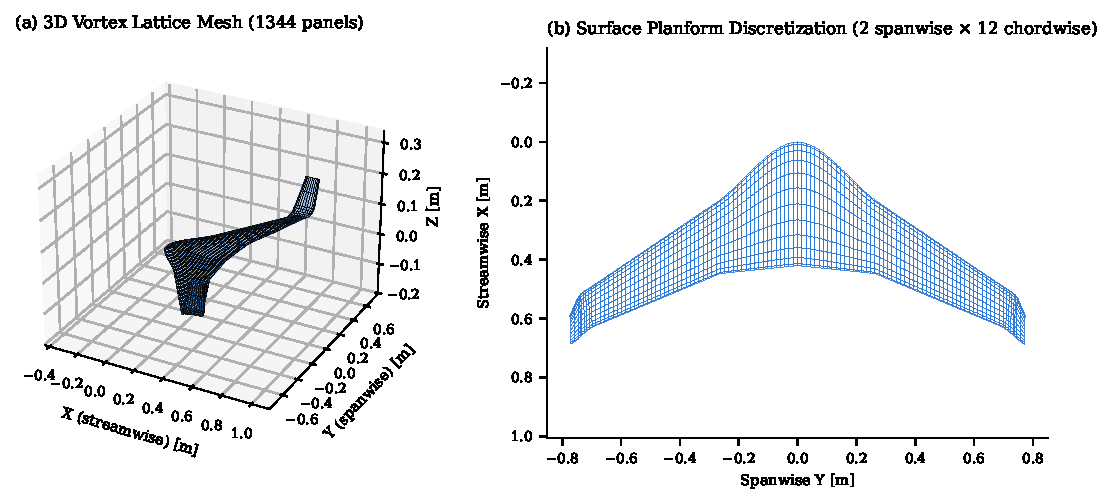
\includegraphics[width=\linewidth]{figures/fig_vlm_discretization.pdf}
\caption{Computational surface panel discretization of the tailless BWB UAV. (a) 3D isometric perspective showing chordwise and spanwise panel distributions across the center-body, outer wing, and canted winglet surfaces. (b) 2D planform projection illustrating cosine panel clustering along the leading and trailing edges ($N_{\mathrm{panels}} = 1{,}344$).}
\label{fig:vlm_discretization}
\end{figure}

As illustrated in Fig.~\ref{fig:vlm_discretization}, the wing is defined by 29 sections per side (25 equally spaced stations on the main wing, three on the circular-arc winglet junction and one at the winglet tip), which gives 28 section intervals. The production discretization uses 2 spanwise panels per interval and 12 chordwise panels, that is 672 panels per side and $1{,}344$ in total ($1{,}152$ on the main wing and $192$ on the winglet junction and winglets).
Chordwise panel distribution employs cosine spacing, clustering panels densely at the leading edge to capture suction peaks and at the trailing edge to enforce the Kutta condition accurately. Spanwise panel boundaries are aligned with structural section breaks to prevent geometric skewness. The sensitivity of aerodynamic coefficients and static margin to panel resolution is formally quantified in the 7-level grid convergence audit of Section~\ref{sec:grid_convergence}.

\subsection{Longitudinal Stability and Trim Derivation}
For unaccelerated level flight at cruise speed $V$, the vehicle must generate the required equilibrium lift coefficient:
\begin{equation}
C_{L,\mathrm{cruise}} = \frac{2 m g}{\rho V^2 S_{\mathrm{ref}}}
\end{equation}
Because the lattice lift is linear in the angle of attack, the pipeline evaluates $C_L$ at $\alpha = 0^\circ$ and $5^\circ$ and interpolates linearly to the angle $\alpha_{\mathrm{cruise}}$ at which $C_L(\alpha_{\mathrm{cruise}}) = C_{L,\mathrm{cruise}}$; a design is rejected if this angle falls outside $[-15^\circ, 20^\circ]$. A third lattice solution at $\alpha_{\mathrm{cruise}}$ gives the forces, the pitching moment about the center of gravity and the stability derivatives.

The longitudinal aerodynamic neutral point $x_{\mathrm{np}}$ follows from the finite-difference stability derivatives that AeroSandbox computes about the cruise point:
\begin{equation}
x_{\mathrm{np}} = x_{\mathrm{ref}} - \bar{c} \cdot \frac{\partial C_m / \partial \alpha}{\partial C_L / \partial \alpha}
\end{equation}
where $x_{\mathrm{ref}}$ is the moment reference point, here the center of gravity $x_{\mathrm{cg}}$, $\bar{c}$ is the mean aerodynamic chord, and $\partial C_m / \partial \alpha$ and $\partial C_L / \partial \alpha$ are the stability derivatives about that point. The longitudinal static margin is then defined non-dimensionally as:
\begin{equation}
SM = \frac{x_{\mathrm{np}} - x_{\mathrm{cg}}}{\bar{c}}
\end{equation}
Constraint Eq.~\eqref{eq:con_sm} enforces $SM \in [0.05, 0.25]$, guaranteeing static pitch stability while preventing excessive pitch stiffness that would degrade maneuvering authority or impose severe trim drag.

\subsection{Viscous Profile Drag and Strip Theory Integration}
Inviscid vortex lattice methods capture induced vortex drag $C_{D,\mathrm{ind}}$ but omit viscous shear stresses and pressure drag arising from boundary-layer development. To capture total cruise drag, the pipeline couples the VLM induced drag with a 2D strip-theory viscous drag integration:
\begin{equation}
C_{D,\mathrm{total}} = C_{D,\mathrm{ind}} + C_{D0} + C_{D,\mathrm{trim}}
\end{equation}
The parasite drag $C_{D0}$ is evaluated by integrating local section profile drag across spanwise strips:
\begin{equation}
C_{D0} = \frac{2}{S_{\mathrm{ref}}} \int_0^{b/2} c(y) \cdot c_{d,\mathrm{profile}}(y) \, dy
\end{equation}
where the local section drag follows a flat-plate skin-friction estimate with a form factor~\cite{raymer2018aircraft}. With the strip Reynolds number $Re_c = V c / \nu$ and the section thickness ratio $\tau$,
\begin{equation}
C_f = x_{\mathrm{tr}}\,\frac{1.328}{\sqrt{x_{\mathrm{tr}} Re_c}} + (1 - x_{\mathrm{tr}})\,\frac{0.455}{(\log_{10} Re_c)^{2.58}}, \qquad c_{d,\mathrm{profile}} = 2\,(1 + 0.2\,\tau)\,\big(1 + 2\tau + 60\tau^4\big)\, C_f
\end{equation}
with an assumed transition location $x_{\mathrm{tr}} = 0.40$ on every strip; the factor $2(1 + 0.2\tau)$ is the wetted-area ratio and the last bracket the form factor. No compressibility correction is applied ($M \approx 0.11$). The skin friction and form drag of the motor boom, motor body and spinner fairing are added in the same way. Trim drag is estimated from the residual cruise pitching moment as $C_{D,\mathrm{trim}} = C_m^2 / (\pi A\!R\, e_{\delta}\, f_{\delta})$ with an elevon effectiveness $e_{\delta} = 0.60$ and an elevon area fraction $f_{\delta} = 0.20$; no control surface is deflected in the lattice model.

\subsection{Independent Models Used for Verification}
\label{sec:mf_tools}
Three tools check the low-order pipeline, and none of them is used inside the optimization: AeroBuildup, the viscous strip method of AeroSandbox; NeuralFoil section polars with predicted transition~\cite{sharpe2024neuralfoil}; and inviscid Euler solutions with SU2~\cite{economon2016su2} on unstructured meshes of about $1.2 \times 10^5$ nodes generated with Gmsh~\cite{geuzaine2009gmsh}. Supplementary Section~\ref{sec:mf_architecture} gives the solver settings. Section~\ref{sec:validation} and Supplementary Sections~\ref{sec:grid_convergence} to~\ref{sec:cfd_validation} use these tools to check the ranking and the constraint values produced by the pipeline.

\section{Clamped Planform Loft, Bound Sensitivity and Mass Balance}
\label{sec:geometric_manifold}

\subsection{Planform Loft and Chord Clamp}
\label{sec:loft_def}
The planform is built from the design vector as follows (Fig.~\ref{fig:geometric_manifold}). Over the center body, $y \in [0, y_b]$ with $\xi = y/y_b$ and $t_\Lambda = \tan\Lambda_{\mathrm{in}}$, the leading edge is a cubic with zero slope at the symmetry plane and the trailing edge is a straight line from the root trailing edge to the blend-station trailing edge:
\begin{equation}
x_{\mathrm{LE}}(y) = t_\Lambda\, y_b\,\big(2\xi^2 - \xi^3\big), \qquad x_{\mathrm{TE}}(y) = c_r + \big(t_\Lambda\, y_b + c_b - c_r\big)\,\xi .
\label{eq:le_te}
\end{equation}
The chord is their difference,
\begin{equation}
c(y) = c_r + y_b\,\big[\, t_\Lambda\,\xi\,(1-\xi)^2 - \delta\,\xi \,\big], \qquad \delta = \frac{c_r - c_b}{y_b},
\label{eq:chord_cb}
\end{equation}
which equals $c_r$ at the root and $c_b$ at the blend station. Outboard of the blend station the leading edge is straight with sweep $\Lambda_{\mathrm{out}}$ and the chord tapers linearly from $c_b$ to $c_t = \lambda c_b$. The leading edge is therefore smooth at the symmetry plane and continuous, with a change of sweep, at the blend station. Twist varies linearly from $\theta_0$ to $\theta_1$ over the center body and piecewise linearly through $\theta_2$ (mid outer wing) to $\theta_t$ at the tip. The section is the MH91 reflexed airfoil at the root (maximum thickness $15.0\%$ of chord), blended linearly into the MH60 airfoil ($10.1\%$) at the blend station and kept constant outboard.

\begin{figure}[htbp]
\centering
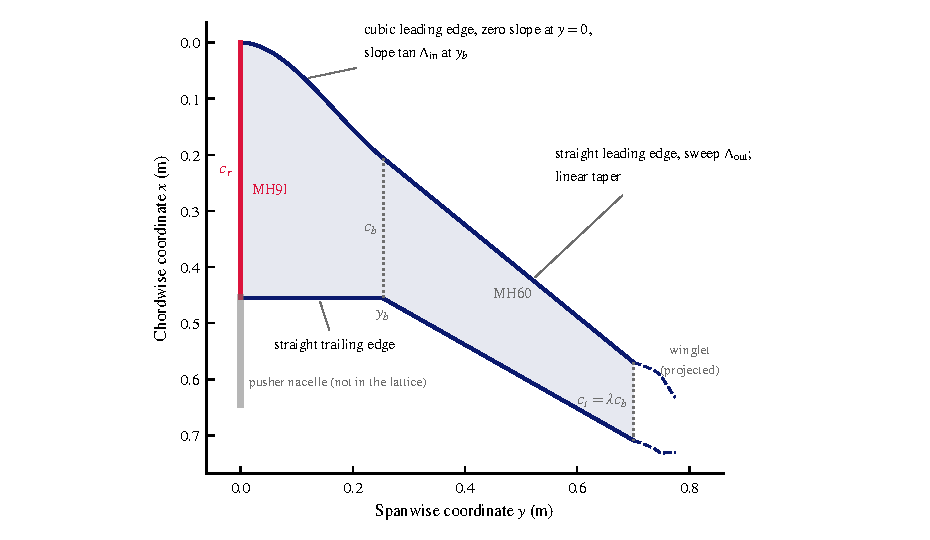
\includegraphics[width=\linewidth]{figures/figure2_geometric_manifold.pdf}
\caption{Planform parameterization: inner and outer leading-edge sweep $\Lambda_{\mathrm{in}}, \Lambda_{\mathrm{out}}$, blend station $y_{b}$, station chords $c_{r}, c_{b}, c_{t}$, the airfoil transition from MH91 to MH60 over the center body, and the pusher nacelle.}
\label{fig:geometric_manifold}
\end{figure}

\paragraph{Clamp} Before lofting, the builder clips the station chords so that they are ordered with a margin of $0.05\,\mathrm{m}$:
\begin{equation}
c_b \leftarrow \min\!\big(\max(c_b,\, 0.25),\; c_r - 0.05\big), \qquad c_t \leftarrow \min\!\big(\max(\lambda c_b,\, 0.05),\; c_b - 0.05\big).
\label{eq:clamp}
\end{equation}
This clamp is what the preprint of this work called a geometric manifold. It guarantees $c_r > c_b > c_t$, so the blend-station chord can never exceed the root chord, and the linear outer taper is monotone.

\paragraph{What the clamp does not guarantee} The clamp orders the three station chords; it does not make the chord monotone between the root and the blend station. Differentiating Eq.~\eqref{eq:chord_cb},
\begin{equation}
\frac{dc}{dy} = t_\Lambda\,(1-\xi)(1-3\xi) - \delta ,
\end{equation}
which is largest at the symmetry plane, where it equals $t_\Lambda - \delta$. The chord is therefore non-increasing over the whole center body if and only if
\begin{equation}
\tan\Lambda_{\mathrm{in}} \;\le\; \frac{c_r - c_b}{y_b},
\label{eq:mono}
\end{equation}
a condition that neither the clamp nor the bounds impose. When it is violated the chord first grows slightly outboard of the root before decreasing. Over the \NvMonoN\ valid designs of the original campaign, \NvMonoViolShare\% violate Eq.~\eqref{eq:mono}; the local growth of the chord has a median of \NvMonoMedian\,mm among them, exceeds $1\,\mathrm{mm}$ in \NvMonoGtOne\% of all valid designs and is at most \NvMonoMax\,mm (about $1\%$ of the root chord). The effect is small, but an earlier version of this manuscript stated a proof of spanwise chord monotonicity; that proof applied to a smoothstep chord law that the bay-volume estimate uses, not to the loft of Eq.~\eqref{eq:le_te} that the aerodynamic model uses, and it is withdrawn.

\subsection{Clamp Activity and Controlled Benchmark}
\label{sec:loft}
A preliminary study of $1{,}000$ Latin hypercube designs with uncoupled chord bounds (Supplementary Section~\ref{sec:ablation_study}) found a lower maximum $L/D$ among chord-inverted planforms, but the difference disappears when the designs are matched by reference area ($p = 0.49$), so that sample gives no evidence that chord inversion by itself lowers the efficiency computed by this pipeline. The controlled test is the following.

Within the bounds of the optimization ($c_{b} \in [0.25, 0.35]\,\mathrm{m}$, $c_{r} \in [0.42, 0.52]\,\mathrm{m}$, $\lambda \ge 0.55$) the clamp of Eq.~\eqref{eq:clamp} can never change a design: the largest blend chord is $0.07\,\mathrm{m}$ below the smallest root chord, and the taper floor keeps the tip chord above $0.05\,\mathrm{m}$ and more than $0.05\,\mathrm{m}$ below the blend chord. In a ten-seed search inside these bounds the clamp condition was met in none of the 2,870 evaluations. The designs reported in this paper were therefore not shaped by the clamp.

\begin{figure}[htbp]
\centering
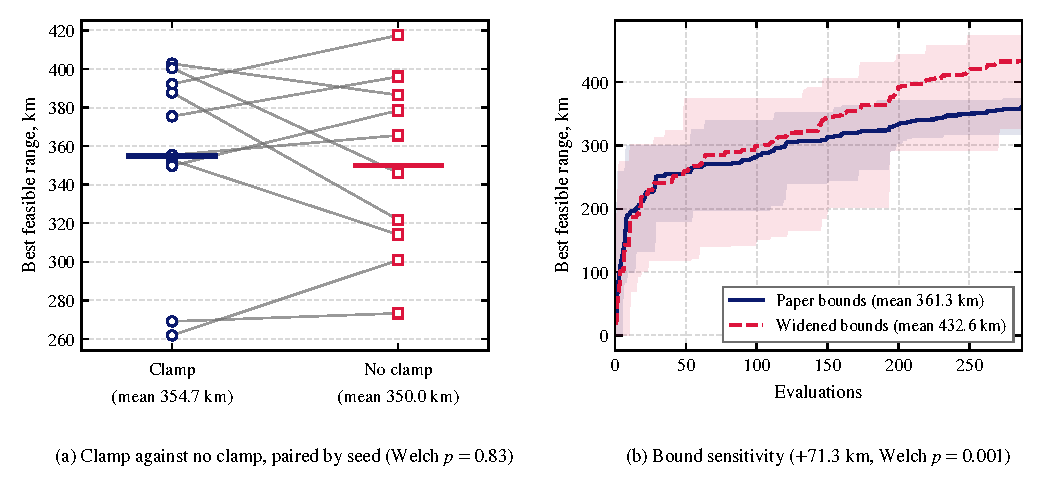
\includegraphics[width=\linewidth]{figures/fig_manifold_bounds.pdf}
\caption{Controlled loft and bound experiments, ten seeds each, 287 evaluations, no pool. (a) Best range of each seed with and without the chord clamp, blend-chord bound widened to $c_b \in [0.15, 0.65]\,\mathrm{m}$; lines join runs with the same seed and bars mark the means. (b) Mean running best with the original bounds and with four bounds relaxed; bands are the minimum-to-maximum envelopes over seeds.}
\label{fig:manifold_bounds}
\end{figure}

To test whether the clamp helps when the bounds do permit inversion, a controlled ten-seed experiment was run with the blend-chord bound widened to $c_{b} \in [0.15, 0.65]\,\mathrm{m}$. Both arms use the same search (48 Latin hypercube designs followed by Gaussian perturbations of the ten best designs found so far, 287 evaluations in total, no pool), the same seeds and the production evaluator; the only difference is that the two clipping lines of Eq.~\eqref{eq:clamp} are removed in the second arm. As presented in Table~\ref{tab:loft} and Fig.~\ref{fig:manifold_bounds}(a), the clamped search achieved a mean range of \NclampMean\,km compared to \NnoclampMean\,km for the unconstrained search ($\Delta = +4.7\,\mathrm{km}$, $p = 0.83$ via Welch's $t$-test and $p = 0.70$ via paired seed test). The clamped search was better in 4 of the 10 paired seeds, and the 95\% interval of the paired difference is about $[-22, +31]\,\mathrm{km}$, so effects of up to about $8\%$ in either direction cannot be excluded by this test.

The evidence therefore supports a limited statement. The clamp is a validity guard on the ordering of the station chords: it is never triggered inside the bounds used for the optimization, and when the bounds are widened until it is triggered in most samples it shows no measurable effect on the best range found. No claim is made that it improves the optimization.

\subsection{Exploration Bound Sensitivity Analysis}
\label{sec:bound_sensitivity}
To measure how much the result depends on the bounds, the same ten-seed search was run inside the bounds of Table~\ref{tab:design_bounds} and with four bounds relaxed, namely those on which the best designs of the original campaign lie: the battery-mass cap ($3.5 \to 4.5\,\mathrm{kg}$), the taper-ratio floor ($0.55 \to 0.35$), the winglet-twist cap ($0^\circ \to +5^\circ$) and the blend-chord cap ($0.35 \to 0.45\,\mathrm{m}$). The cruise-speed floor is a mission requirement and was not relaxed.

As reported in Table~\ref{tab:loft} and Fig.~\ref{fig:manifold_bounds}(b), relaxing the exploration bounds increased the mean discovered operational range from \NpaperBndMean\,km to \NwideBndMean\,km, a gain of $71.3$\,km ($+19.7\%$, Welch $p = 0.001$), with the best run reaching \NwideBndMax\,km. These runs use a simple elite search without the pool, so their absolute values are not comparable with Table~\ref{tab:budget}; only the difference between the two arms is interpreted.

The best designs are thus limited by the bounds and are not interior optima; no global optimality is claimed. Table~\ref{tab:bound} shows on which bounds the twenty best designs of the original database lie, and Section~\ref{sec:bound_prices} measures the range cost of the individual bounds, of which only the battery-mass cap turns out to be measurable.

\subsection{Mass and Center-of-Gravity Build-Up and Trim Constraints}
\label{sec:dynamic_balance}
Longitudinal equilibrium for a tailless aircraft requires satisfying the moment equation~\cite{nelson1998flight}:
\begin{equation}
C_m(\alpha) = C_{m0} + \left(\frac{x_{\mathrm{cg}} - x_{\mathrm{np}}}{\bar{c}}\right) C_L(\alpha)
\end{equation}
To achieve trimmed flight ($C_m = 0$) at cruise lift $C_{L,\mathrm{cruise}}$ without deploying elevon control surfaces, the planform must generate a positive zero-lift pitching moment:
\begin{equation}
C_{m0} = SM \cdot C_{L,\mathrm{cruise}} > 0
\label{eq:trim_req}
\end{equation}
This positive moment is synthesized through reflexed airfoil camber combined with negative wingtip twist ($\theta_t \in [-12^\circ, -2^\circ]$).

\begin{figure}[htbp]
\centering
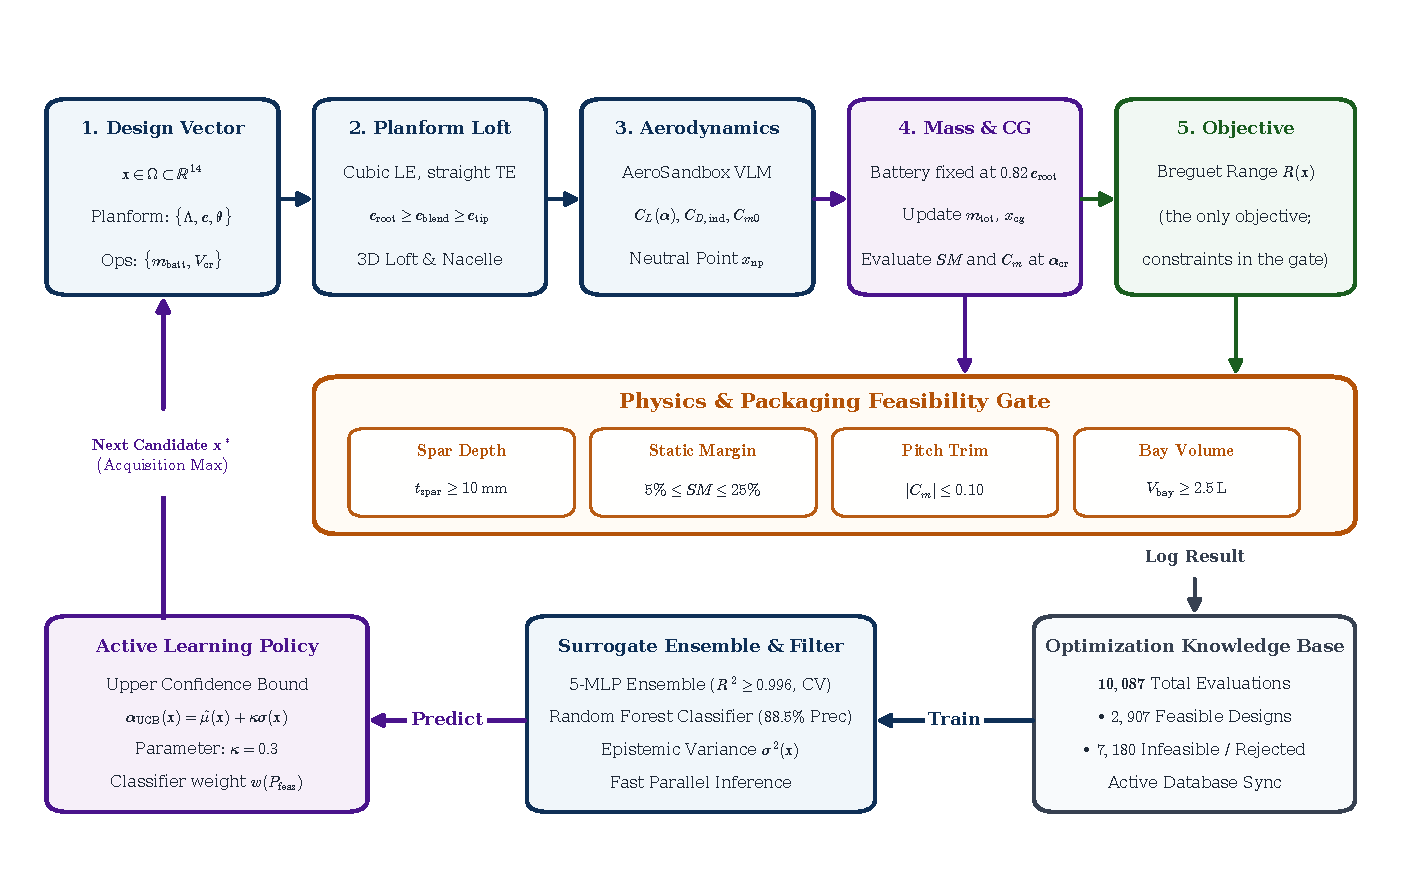
\includegraphics[width=0.92\linewidth]{figures/figure3_trim_loop_architecture.pdf}
\caption{Evaluation and search architecture. For every design vector the evaluator builds the clamped planform, runs the VLM, recomputes total mass and center of gravity with the battery centroid fixed at $0.82\,c_{r}$, and checks the static-margin, trim, spar-depth and bay-volume constraints. The classifier and surrogate ensemble then guide the active-learning acquisition. No battery position is solved for inside the loop.}
\label{fig:trim_loop_architecture}
\end{figure}

Every evaluation recomputes the total mass and center of gravity from the design vector (Fig.~\ref{fig:trim_loop_architecture}). The payload (at $0.20\,c_{r}$), avionics (at $0.25\,c_{r}$) and motor (at $c_{r} + 0.02\,\mathrm{m}$) are fixed point masses, the airframe mass $1.0 + 1.5\,S_{\mathrm{ref}}$\,kg acts at $0.40$ MAC behind the MAC leading edge, and the battery mass $m_{\mathrm{b}}$ is a design variable. The battery centroid is held fixed at $x_{\mathrm{batt}} = 0.82\,c_{r}$ ($f_{b} = 0.82$) for every design:
\begin{equation}
x_{\mathrm{cg}} = \frac{\sum_i m_i x_i + m_{\mathrm{b}}\, x_{\mathrm{batt}}}{m_{\mathrm{total}}}, \qquad x_{\mathrm{batt}} = 0.82\,c_{r}.
\end{equation}
The battery position is therefore an input to the optimization and not a quantity solved for: the evaluator contains no inversion for $x_{\mathrm{batt}}$. The static margin follows from the VLM-computed neutral point $x_{\mathrm{np}}$ and this center of gravity, $SM = (x_{\mathrm{np}} - x_{\mathrm{cg}})/\bar{c}$. A design is feasible only if $SM \in [0.05, 0.25]$ and $|C_m| \le 0.10$ at cruise (hard constraints), the center-body volume exceeds $2.5\,\mathrm{L}$ ($g_6$) and the spar depth is at least $10\,\mathrm{mm}$; a center of gravity outside $15$ to $40\%$ MAC is penalized softly. For the best design of the original campaign these constraints give natural pitch trim ($C_m = -0.019$) with $SM = 22.5\%$ and near-zero trim drag ($1.1\%$ of total drag). Table~\ref{tab:mass} shows how range and static margin change when the airframe mass model is scaled by $0.7$ and $1.3$, and Section~\ref{sec:robustness} reports the sensitivity of the best designs of all search arms to the battery position and mass.

A post-hoc inversion of the same moment balance is available for a single design, for example to ask which battery position would give a target static margin $SM^{\ast}$, with $x_{\mathrm{cg,target}} = x_{\mathrm{np}} - SM^{\ast}\bar{c}$:
\begin{equation}
x_{\mathrm{batt}} = \frac{m_{\mathrm{total}}\, x_{\mathrm{cg,target}} - \sum_i m_i x_i}{m_{\mathrm{b}}}.
\end{equation}
This inversion was applied after the optimization to the best design of the original campaign only. Fig.~\ref{fig:trim_sensitivity} is the corresponding post-hoc battery-position sweep and shows the feasible corridor around the chosen value of $0.82\,c_{r}$.

\begin{figure}[htbp]
\centering
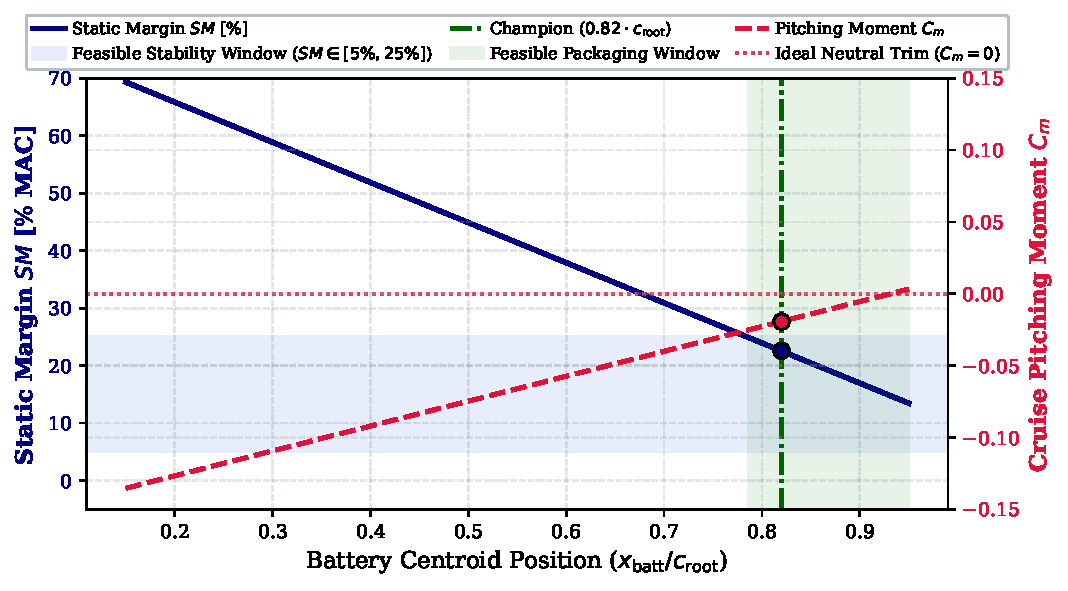
\includegraphics[width=0.95\linewidth]{figures/figure4_trim_sensitivity.pdf}
\caption{Post-hoc battery-position sweep on the original-campaign champion geometry: longitudinal trim and static stability as a function of battery centroid position ($x_{\mathrm{batt}} / c_{r}$), with all other mass moments held fixed. The feasible corridor ($SM \in [5\%, 25\%]$, $|C_m| \le 0.10$) spans $x_{\mathrm{batt}}/c_r$ from $0.79$ to $0.95$. The optimization fixes the battery at $0.82 \cdot c_{r}$ (green vertical line), which lies inside this corridor and gives $SM = 22.5\%$ and near-zero natural trim ($C_m = -0.019$).}
\label{fig:trim_sensitivity}
\end{figure}


\section{Equal-Budget Benchmark Protocol and Surrogate Framework}
\label{sec:protocol}

\subsection{Surrogate Ensemble and Cross-Validation}
The active-learning loop uses an ensemble of $M = 5$ multi-layer perceptrons (scikit-learn \texttt{MLPRegressor}), each with two hidden layers of 64 rectified-linear units, trained with Adam for at most 1{,}000 epochs with early stopping on a held-out $10\%$ of the training data. Inputs are scaled to $[0, 1]$ and outputs are standardized. Each network predicts five quantities jointly: $C_L$, $C_D$, $L/D$, the calm-air range $R$ and the soft-penalty score of Section~\ref{sec:formulation}. The ensemble is fitted on feasible designs only, because infeasible designs carry no aerodynamic outputs. The five members differ only in their random seed ($42, 101, 2024, 777, 999$ in the original campaign; $42 + 7s + 100i$, $i = 0,\ldots,4$, in replication $s$). The prediction and its uncertainty are the ensemble mean and standard deviation,
\begin{equation}
\bar{\mu}_y(\mathbf{x}) = \frac{1}{M} \sum_{m=1}^M \hat{y}_m(\mathbf{x}), \qquad \bar{\sigma}_y(\mathbf{x}) = \sqrt{\frac{1}{M} \sum_{m=1}^M \big(\hat{y}_m(\mathbf{x}) - \bar{\mu}_y(\mathbf{x})\big)^2} .
\end{equation}
Five-fold cross-validation on the feasible designs of the database gives $R^2 \ge 0.996$ for every target and a mean absolute percentage error of $2.3\%$ for range (Table~\ref{tab:cv}). These are in-distribution figures; Section~\ref{sec:distribution_shift} shows that accuracy is much lower on the designs that the loop itself proposes.

\subsection{Feasibility Classifier and Recall Audit}
\label{sec:classifier_audit}
About $72\%$ of the space-filling pool is infeasible. A random forest classifier with $100$ trees~\cite{breiman2001random} is therefore trained on all evaluated designs, feasible or not, to predict a probability of feasibility $\mathcal{P}_{\mathrm{feas}}(\mathbf{x}) \in [0, 1]$, which weights the acquisition function below. An infeasible design returns no aerodynamic outputs, so from the point of view of the search the constraints act as what the simulation-optimization literature calls hidden constraints~\cite{ledigabel2015taxonomy}, and a model of the probability that an evaluation succeeds is the usual way to handle them in surrogate-based aircraft design~\cite{bussemaker2024hidden}.

The held-out performance of this classifier was audited on the $\NclfNrows$-evaluation database with five repeated stratified 80/20 random splits (seeds 0 to 4) and one scaled-feature forest (Table~\ref{tab:classifier_audit}):
\begin{itemize}
    \item \textbf{Global and frontier recall.} Precision is $\NfnPrec\% \pm \NfnPrecSd\%$ and recall is $\NfnRecall\% \pm \NfnRecallSd\%$ at a threshold of $0.5$ (the same forest without feature scaling gives $\NfnRecallUnscaled\%$ recall); $\NclfInfeasShare\%$ of the audited designs are infeasible. Recall is higher among good designs: $\NfnTenRecall\% \pm \NfnTenRecallSd\%$ among the top 10\% of valid designs ($R \ge \NclfQten\,\mathrm{km}$) and $\NfnTwoRecall\% \pm \NfnTwoRecallSd\%$ among the top 2\% ($R \ge \NclfQtwo\,\mathrm{km}$), the latter on only \NfnTwoN\ designs per split.
    \item \textbf{Where the false negatives lie.} $\NfnWithin\%$ of the falsely rejected valid designs lie within $10\%$ of the static-margin or trim limits, against $\NtpWithin\%$ of the correctly accepted ones. Their median range is $\NfnMedian\,\mathrm{km}$ (accepted: $\NtpMedian\,\mathrm{km}$), but the best falsely rejected design averages $\NfnMax\,\mathrm{km}$ over the splits (maximum $\NfnMaxSplit\,\mathrm{km}$). The decision boundary therefore passes close to the best designs, and a hard gate at $0.5$ would exclude some of them.
    \item \textbf{What the classifier cannot see.} The forest is trained on axis-aligned splits of the raw design variables. The washout rule $g_8$ is a relation between four variables, and Section~\ref{sec:budget_results} shows that the classifier-weighted search still proposes designs that violate it.
\end{itemize}

\subsection{Acquisition Function and Active-Learning Loop}
\label{sec:al_loop}
Candidates are ranked by an upper confidence bound on range~\cite{srinivas2012information}, weighted by the classifier~\cite{gelbart2014bayesian} and reduced by the predicted soft penalty:
\begin{equation}
a(\mathbf{x}) = \big( \bar{\mu}_R(\mathbf{x}) + \kappa\, \bar{\sigma}_R(\mathbf{x}) \big)\, w\!\big(\mathcal{P}_{\mathrm{feas}}(\mathbf{x})\big) - \max\!\big(0, \bar{\mu}_{\pi}(\mathbf{x})\big), \qquad w(p) = \frac{1}{1 + e^{-10\,(p - 0.5)}} ,
\label{eq:ucb_acquisition}
\end{equation}
with $\kappa = 0.3$ in the original campaign and in every run reported here. The weight $w$ is a sigmoid of the classifier probability; it equals $0.5$ at $\mathcal{P}_{\mathrm{feas}} = 0.5$ and saturates toward $0$ and $1$. Probability-of-feasibility weighting of this kind has known limitations~\cite{cordelier2026multifidelity}, and Section~\ref{sec:feas_ablation} tests it by replacing $w$ with a hard $0/1$ gate at $0.5$ and by removing it ($w \equiv 1$).

One cycle of the loop proceeds as follows. (i) The ensemble is refitted on all feasible designs and the classifier on all designs evaluated so far, including the pool. (ii) The acquisition $a(\mathbf{x})$ is maximized over the box of Table~\ref{tab:design_bounds} by differential evolution (SciPy, population $150 \times 14 = 2{,}100$, at most 300 generations, initial population seeded with the 20 best feasible designs, followed by the default local polish). (iii) From the final population, the five distinct members with the highest acquisition and one further member with the largest weighted uncertainty $\bar{\sigma}_R\, w$ are taken as candidates; candidates that duplicate an evaluated design are dropped. (iv) The candidates are evaluated with the full pipeline and added to the data. The loop therefore proposes up to six designs per cycle and retrains every cycle. The original campaign ran this loop until a wall-clock limit, which it reached after 287 evaluations; the replications run it for exactly 287 evaluations instead, so that every strategy has the same budget.

\subsection{Equal-Budget Protocol}
\label{sec:budget_protocol}
Figure~\ref{fig:protocol} summarizes the benchmark. Every strategy starts from the same pool of 9{,}800 Latin hypercube designs (best range $352.9\,\mathrm{km}$, $28.1\%$ feasible) and may spend $287$ further evaluations of the full pipeline. A run is one strategy with one random seed. The strategies are:
\begin{enumerate}
    \item \textbf{Active learning as published (AL).} The loop of Section~\ref{sec:al_loop}, ten replications (seeds 0 to 9) plus the original campaign. The published loop evaluates the candidates exactly as the differential evolution returns them.
    \item \textbf{Active learning with washout repair (AL-R).} The same loop, except that the four twist variables of each candidate are sorted into the order required by $g_8$ before the duplicate check and the evaluation (\NvNALR\ seeds). Every other strategy below, and the pool itself, already applies this sorting; Section~\ref{sec:budget_results} explains why this arm was added.
    \item \textbf{Trust-region Bayesian optimization (TuRBO).} A TuRBO-1 implementation~\cite{eriksson2019turbo}: a Gaussian process (Mat\'ern-$5/2$ kernel with automatic relevance determination) is fitted to at most 400 designs inside a trust region centered on the best feasible design, with infeasible designs assigned the worst feasible value in the region; batches of six are chosen by Thompson sampling over 2{,}000 Sobol candidates with the TuRBO perturbation mask; the region side (initially $0.4$ of the normalized range) doubles after three consecutive improving batches, halves after five consecutive failures and restarts below $0.01$ (\NvNTurbo\ seeds).
    \item \textbf{Adaptive local search (adapt10).} No surrogate. Each batch of six consists of Gaussian perturbations, with a standard deviation of $10\%$ of each variable's range, of randomly chosen members of the current 20 best feasible designs (pool and new evaluations together), so that the set of parents moves as better designs are found (\NvNAdapt\ seeds). This arm has the same batch structure and the same parent set as the active-learning loop but replaces the surrogate-optimized proposals by random ones.
    \item \textbf{Static local search (local10, local5).} Gaussian perturbations ($10\%$ or $5\%$ of the range) of randomly chosen members of the 20 best pool designs; the parent set never changes (10 seeds each).
    \item \textbf{Fresh Latin hypercube and uniform random sampling.} 287 new space-filling or uniform samples in the full box (10 seeds each).
\end{enumerate}
Section~\ref{sec:pool_size} repeats TuRBO, adapt10 and AL-R from random subsamples of 288, 1{,}000 and 3{,}000 pool designs. Three further arms isolate the classifier weight (Section~\ref{sec:feas_ablation}): active learning with a hard gate, active learning without the weight (each with and without the washout repair where stated), and TuRBO with the sigmoid weight applied to its Thompson samples.

\begin{figure}[htbp]
\centering
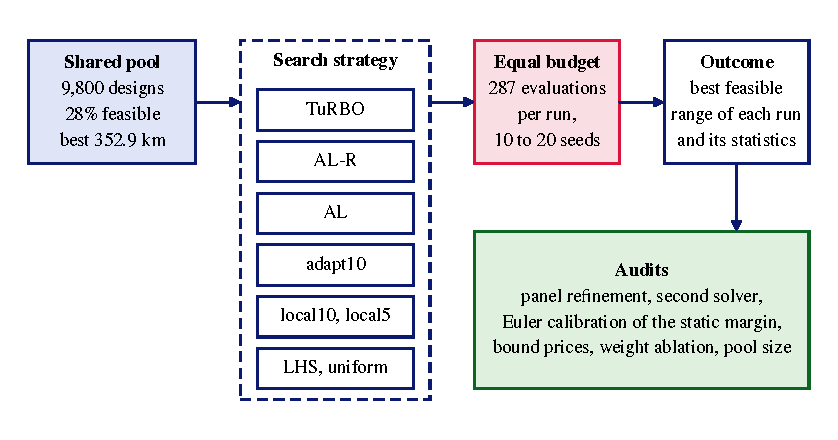
\includegraphics[width=\linewidth]{figures/fig_protocol.pdf}
\caption{Structure of the benchmark. All strategies share the pool, the evaluator and the budget; they differ only in how the 287 further designs are proposed. The audits are reported in Section~\ref{sec:results}.}
\label{fig:protocol}
\end{figure}

\paragraph{Two corrections made during the audit of the benchmark code} Both are reported because they change numbers, and the runs made before each correction are retained and listed in Table~\ref{tab:asrun}. First, the published active-learning loop was the only strategy that did not sort the twist variables, so it alone spent evaluations on designs that fail $g_8$; the AL-R arm removes that asymmetry. Second, the first implementations of TuRBO and of the adaptive local search compared the ranges of new evaluations and of pool designs on two different energy bases (a constant factor of $1.30$ in favor of new designs), which distorted the choice of the trust-region center and of the parent set. Both strategies were rerun with one consistent basis, and the corrected runs are the ones reported as TuRBO and adapt10. The weighting and bound-price experiments of Sections~\ref{sec:feas_ablation} and~\ref{sec:bound_prices}, first made with the first TuRBO implementation, were repeated with the corrected one, and the repeated runs are the ones reported.

\paragraph{Statistics} The outcome of a run is its best feasible range after 287 evaluations. An active-learning run ends early if 40 consecutive cycles produce no candidate that has not already been evaluated; such a run keeps the best value it reached and is not excluded (one AL run stopped at 117 evaluations and one AL-R run at 83). Strategies are compared with two-sided Welch $t$-tests and two-sided Mann--Whitney $U$ tests on these values, and with a percentile bootstrap interval ($20{,}000$ resamples) on the difference of means. For the \NvNfamily\ headline comparisons of Table~\ref{tab:tests} the Welch $p$-values are also reported after Holm correction. A non-significant difference is not read as equivalence; the confidence interval states which differences remain possible. All ranges are on the $\NeU\,\mathrm{Wh/kg}$ basis.

\section{Results, Statistical Benchmark, and Aerodynamic Validation}
\label{sec:results}

\subsection{Equal-Budget Search Benchmark Outcomes}
\label{sec:budget_results}
Table~\ref{tab:budget} and Fig.~\ref{fig:equal_budget} report every strategy of Section~\ref{sec:budget_protocol} after 287 evaluations beyond the shared pool, whose best feasible design reaches \NvPool\,km. Table~\ref{tab:tests} gives the \NvNfamily\ headline comparisons, which Fig.~\ref{fig:forest} shows with their intervals.

\begin{table}[htbp]
\centering\small
\caption{Equal-budget search performance on the shared 9,800-design pool; strategy names as in Section~\ref{sec:budget_protocol}. Range: mean running best after 100 evaluations (pool included), mean $\pm$ standard deviation of the best feasible range after 287 evaluations, and its extremes over runs. Evaluations: share that is feasible over the whole run (valid) and over the first 60 evaluations (valid$_{60}$), and share spent on designs that violate the washout ordering (fail $g_8$). Beating the pool: number of runs that exceed the best pool design and the median number of evaluations needed. One AL run and one AL-R run stopped early by exhaustion and are included with the value they reached.}
\label{tab:budget}
\begin{tabular*}{\linewidth}{@{\extracolsep{\fill}}lrrrrrrrrr@{}}
\toprule
 & & \multicolumn{3}{c}{Best feasible range (km)} & \multicolumn{3}{c}{Share of evaluations (\%)} & \multicolumn{2}{c}{Beating the pool} \\
\cmidrule(lr){3-5}\cmidrule(lr){6-8}\cmidrule(l){9-10}
Strategy & Runs & at 100 & at 287 & min to max & valid & valid$_{60}$ & fail $g_8$ & runs & evals \\
\midrule
TuRBO & 20 & 382.9 & 396.8 $\pm$ 4.4 & 385.3 to 403.0 & 82 & 80 & 0 & 20/20 & 2 \\
AL-R & 20 & 378.8 & 391.5 $\pm$ 6.6 & 367.9 to 399.5 & 64 & 24 & 0 & 20/20 & 31 \\
AL & 11 & 374.1 & 385.0 $\pm$ 10.4 & 368.9 to 397.4 & 59 & 14 & 17 & 11/11 & 43 \\
adapt10 & 20 & 372.9 & 386.1 $\pm$ 6.3 & 369.2 to 393.2 & 68 & 69 & 0 & 20/20 & 34 \\
local10 & 10 & 358.8 & 365.2 $\pm$ 4.7 & 358.5 to 373.1 & 64 & 60 & 0 & 10/10 & 36 \\
local5 & 10 & 359.3 & 364.2 $\pm$ 6.6 & 351.9 to 373.2 & 81 & 80 & 0 & 9/10 & 31 \\
LHS & 10 & 352.9 & 298.3 $\pm$ 27.2 & 260.2 to 337.3 & 28 & 30 & 0 & 0/10 & n/a \\
Uniform & 10 & 352.9 & 307.6 $\pm$ 30.5 & 264.2 to 353.3 & 28 & 26 & 0 & 1/10 & 147 \\
\midrule
Pool only & n/a & n/a & 352.9 & n/a & 28 & n/a & 0 & n/a & n/a \\
\bottomrule
\end{tabular*}

\end{table}

\begin{figure}[htbp]
\centering
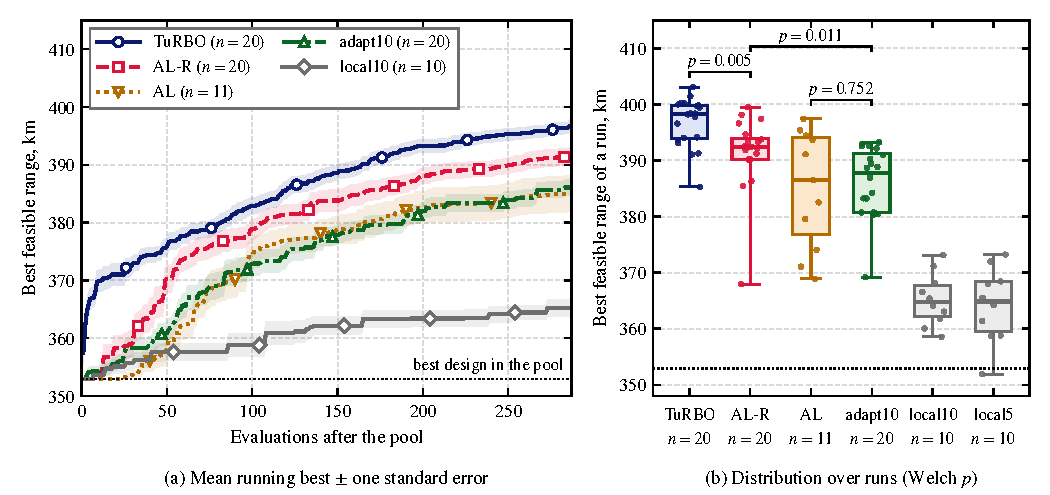
\includegraphics[width=\linewidth]{figures/fig_equal_budget.pdf}
\caption{Equal-budget benchmark. (a) Mean running best feasible range, pool included, against the number of evaluations beyond the pool for the five leading strategies; the bands are $\pm$ one standard error over seeds and the dotted line is the best design in the pool. (b) Best feasible range of every run (dots) for the six strategies that improve on the pool; the box spans the quartiles, the line is the median and the whiskers reach the extremes. Brackets give two-sided Welch $p$-values, not corrected for multiplicity (Table~\ref{tab:tests} gives the corrected values). Fresh Latin hypercube and uniform sampling end below the pool best and are listed in Table~\ref{tab:budget} only.}
\label{fig:equal_budget}
\end{figure}

\begin{table}[htbp]
\centering\small
\caption{Headline comparisons of best feasible range after 287 evaluations. Welch and Mann--Whitney tests are two-sided; Holm correction is applied over the \NvNfamily\ rows; M--W is the Mann--Whitney test; the interval is a percentile bootstrap on the difference of means; $P(A{>}B)$ is the share of run pairs in which $A$ ends above $B$.}
\label{tab:tests}
\begin{tabular*}{\linewidth}{@{\extracolsep{\fill}}lcrrrrrcr@{}}
\toprule
 & & \multicolumn{2}{c}{Difference} & \multicolumn{3}{c}{Two-sided $p$} & & \\
\cmidrule(lr){3-4}\cmidrule(lr){5-7}
$A$ minus $B$ & $n_A$, $n_B$ & km & \% & Welch & Holm & M--W & 95\% CI (km) & $P(A{>}B)$ \\
\midrule
TuRBO $-$ AL-R & 20, 20 & $+5.3$ & $+1.4$ & 0.005 & 0.020 & 0.001 & $[2.2,\ 8.8]$ & 0.80 \\
AL-R $-$ AL & 20, 11 & $+6.5$ & $+1.7$ & 0.079 & 0.159 & 0.180 & $[0.1,\ 12.9]$ & 0.65 \\
AL-R $-$ adapt10 & 20, 20 & $+5.4$ & $+1.4$ & 0.011 & 0.033 & 0.003 & $[1.4,\ 9.2]$ & 0.78 \\
TuRBO $-$ adapt10 & 20, 20 & $+10.7$ & $+2.8$ & $<$0.001 & $<$0.001 & $<$0.001 & $[7.5,\ 14.1]$ & 0.94 \\
AL $-$ adapt10 & 11, 20 & ${-}1.1$ & ${-}0.3$ & 0.752 & 0.752 & 0.918 & $[-7.6,\ 5.1]$ & 0.51 \\
adapt10 $-$ local10 & 20, 10 & $+20.9$ & $+5.7$ & $<$0.001 & $<$0.001 & $<$0.001 & $[16.9,\ 24.6]$ & 0.99 \\
AL $-$ local10 & 11, 10 & $+19.8$ & $+5.4$ & $<$0.001 & $<$0.001 & $<$0.001 & $[13.2,\ 26.1]$ & 0.96 \\
\bottomrule
\end{tabular*}

\end{table}

Four results follow.

\textbf{TuRBO is the strongest strategy.} It reaches $\NvMeanTurbo \pm \NvSdTurbo$\,km over \NvNTurbo\ seeds, \NvGainPctTurbo\% above the pool best, with the highest feasible fraction (\NvValidTurbo\%) and an improvement on the pool within the first few evaluations of every run. It exceeds the adaptive local search by \NvDTurbovAdapt\,km (Holm $p \NvHTurbovAdapt$) and the published active-learning loop by \NvDTurbovAL\,km (Welch $p \NvPTurbovAL$, bootstrap 95\% interval $\NvCITurbovAL$\,km).

\textbf{Active learning with the washout repair is second.} AL-R reaches $\NvMeanALR \pm \NvSdALR$\,km over \NvNALR\ seeds. TuRBO leads it by \NvDTurbovALR\,km (\NvPctTurbovALR\%; Welch $p \NvPTurbovALR$, Mann--Whitney $p \NvUTurbovALR$, Holm $p \NvHTurbovALR$; interval $\NvCITurbovALR$\,km), a lead that remains significant after Holm correction. The size of the lead depends on one run: AL-R seed 16 exhausted its candidate list after 83 evaluations at \NvMinALR\,km. Without that run AL-R averages $\NvMeanALRc \pm \NvSdALRc$\,km and the gap to TuRBO is \NvDTurbovALRc\,km (Welch $p \NvPTurbovALRc$, interval $\NvCITurbovALRc$\,km). Early exhaustion occurred in one of \NvNALR\ AL-R runs and one of \NvNAL\ AL runs and in no run of any other strategy; it is a reliability cost of the surrogate loop and is kept in the headline numbers. AL-R exceeds the adaptive local search by \NvDALRvAdapt\,km (Holm $p \NvHALRvAdapt$).

\textbf{The published active-learning loop is not better than a surrogate-free adaptive local search.} AL reaches $\NvMeanAL \pm \NvSdAL$\,km and adapt10 $\NvMeanAdapt \pm \NvSdAdapt$\,km; the difference is $\NvDsALvAdapt$\,km (Welch $p \NvPALvAdapt$, interval $\NvCIALvAdapt$\,km). The loop spent \NvWashAL\% of its evaluations on designs that fail the washout ordering $g_8$, which no other strategy could propose. Removing that asymmetry raises the mean by \NvDALRvAL\,km (Welch $p \NvPALRvAL$, Holm $p \NvHALRvAL$) and, on the ten matched seeds analyzed in Section~\ref{sec:feas_ablation}, by \NvDALRtenvALrep\,km (Welch $p \NvPALRtenvALrep$). The surrogate therefore earns a measurable margin over random proposals around the same parent set only once the loop is prevented from proposing designs that a one-line repair would fix.

\textbf{Moving the search center matters more than the surrogate.} Static local search around the 20 best pool designs reaches $\NvMeanLocTen \pm \NvSdLocTen$\,km, and letting the parent set follow new discoveries adds \NvDAdaptvLocTen\,km (Holm $p \NvHAdaptvLocTen$). Measured against the gain of TuRBO over the pool best, static local search recovers \NvShareLocTen\%, adaptive local search \NvShareAdapt\%, published active learning \NvShareAL\%, and AL-R \NvShareALR\%. Fresh Latin hypercube and uniform sampling do not improve on the pool in a 287-evaluation allocation except in one uniform run.

\textbf{The ordering does not depend on where the budget is cut.} Table~\ref{tab:anytime} repeats the comparison at 50, 100, 150 and 200 evaluations. TuRBO has the highest mean and AL-R the second highest at every budget; the lead of TuRBO over AL-R is between \NlAnyTRlo\ and \NlAnyTRhi\,km and reaches the 5\% level (uncorrected) from \NlAnyTRsigFrom\ evaluations onward, and AL-R exceeds the adaptive local search at every budget (Welch $p \le \NlAnyRApmax$). The published loop and the adaptive local search remain within a few kilometers of each other throughout.

\textbf{Doubling the budget narrows the gaps but keeps the ordering.} TuRBO and the adaptive local search (seeds 0 to 9) and AL-R (seeds 0 to 4) were continued from 287 to \NlBudget\ evaluations (Table~\ref{tab:long}). TuRBO reaches $\NlTurboCMean \pm \NlTurboCSd$\,km, the adaptive local search $\NlAdaptCMean \pm \NlAdaptCSd$\,km and AL-R $\NlALRCMean \pm \NlALRCSd$\,km. The second 287 evaluations add \NlTurboGain\,km for TuRBO and \NlAdaptGain\,km for the adaptive local search, so on these ten seeds the lead of TuRBO over the surrogate-free search falls from \NlTvAAD\ to \NlTvACD\,km (Welch $p = \NlTvACP$), while its lead over AL-R on the five shared seeds is \NlTvRCD\,km ($p = \NlTvRCP$). No run of any strategy exceeds \NlAllMax\,km within the original bounds. The strategies therefore approach a common ceiling, which Section~\ref{sec:bound_prices} attributes to the bounds, and the advantage of a model is largest when evaluations are scarce.

\begin{table}[htbp]
\centering\small
\caption{Best feasible range (km, mean $\pm$ standard deviation, pool included) when the runs are continued to twice the budget, and differences between strategies with two-sided Welch $p$-values (not corrected for multiplicity).}
\label{tab:long}
% generated by make_numbers_long.py; do not edit
\begin{tabular*}{\linewidth}{@{\extracolsep{\fill}}lrrr@{}}
\toprule
Evaluations beyond the pool & 287 & 400 & 574 \\
\midrule
TuRBO ($n=10$) & 396.3 $\pm$ 5.3 & 399.2 $\pm$ 4.5 & 400.9 $\pm$ 3.8 \\
AL-R ($n=5$) & 394.8 $\pm$ 3.2 & 395.7 $\pm$ 3.5 & 397.0 $\pm$ 4.1 \\
adapt10 ($n=10$) & 386.1 $\pm$ 7.7 & 391.9 $\pm$ 7.6 & 395.4 $\pm$ 5.7 \\
\midrule
TuRBO minus adapt10, km (Welch $p$) & $+10.2$ (0.003) & $+7.3$ (0.020) & $+5.5$ (0.022) \\
TuRBO minus AL-R, seeds 0 to 4, km (Welch $p$) & $+3.3$ (0.201) & $+4.5$ (0.066) & $+5.8$ (0.031) \\
AL-R minus adapt10, seeds 0 to 4, km (Welch $p$) & $+11.6$ (0.058) & $+5.9$ (0.273) & $+4.3$ (0.286) \\
\bottomrule
\end{tabular*}

\end{table}

Table~\ref{tab:asrun} lists the corrected baselines beside their first implementations. For TuRBO the correction of the energy basis changes the mean by $\NvPairedTurboD$\,km (paired over the same \NvPairedTurboN\ seeds, $p \NvPairedTurboP$), because every trust region starts from a new evaluation within its first batches and then compares new evaluations with each other. For the adaptive local search it raises the mean by \NvDAdaptvAdaptOld\,km (Welch $p \NvPAdaptvAdaptOld$): the first implementation kept too many early evaluations in the parent set. The correction therefore strengthens the surrogate-free baseline that the active-learning loop is compared with.

\subsection{Sensitivity to the Size of the Initial Pool}
\label{sec:pool_size}
The benchmark above shares one pool of 9{,}800 designs, which is $97\%$ of all evaluations. To test whether the conclusions depend on that pool, TuRBO, the adaptive local search and AL-R were rerun from random subsamples of 288, 1{,}000 and 3{,}000 pool designs, with the same 287 further evaluations. The subsample is drawn with a seed tied to the run seed, so the three strategies start from the same designs in runs with the same seed. The outcome of a run is the best feasible range among its subsample and its own evaluations (Table~\ref{tab:pool}, Fig.~\ref{fig:pool_size}).

\begin{table}[htbp]
\centering\small
\caption{Best feasible range (km, mean $\pm$ standard deviation) after 287 evaluations from pools of different size. TuRBO and adapt10: seeds 0 to 9; AL-R: seeds 0 to 4. The last row repeats the runs of the main benchmark with the same seeds. ``Pool best'' is the mean best design of the subsamples. The row marked independent uses ten separately generated 1{,}000-design pools, one per seed, in place of subsamples.}
\label{tab:pool}
\resizebox{\linewidth}{!}{%
% generated by make_numbers_pool.py; do not edit
\begin{tabular}{@{}rrrrrrrr@{}}
\toprule
Pool size & Total evaluations & Pool best (km) & TuRBO (km) & adapt10 (km) & AL-R (km) & TuRBO minus adapt10 (km) & Welch $p$ \\
\midrule
288 & 575 & 295.8 & 388.0 $\pm$ 9.0 & 374.5 $\pm$ 8.4 & 386.1 $\pm$ 5.4 & $+13.5$ & 0.003 \\
1{,}000 & 1{,}287 & 330.3 & 394.2 $\pm$ 5.8 & 377.4 $\pm$ 8.7 & 392.4 $\pm$ 7.1 & $+16.9$ & <0.001 \\
3{,}000 & 3{,}287 & 338.5 & 393.5 $\pm$ 9.1 & 382.4 $\pm$ 8.4 & 390.1 $\pm$ 5.3 & $+11.0$ & 0.011 \\
9{,}800 & 10{,}087 & 352.9 & 396.3 $\pm$ 5.3 & 386.1 $\pm$ 7.7 & 394.8 $\pm$ 3.2 & $+10.2$ & 0.003 \\
\midrule
1{,}000, independent & 1{,}287 & 313.1 & 388.3 $\pm$ 10.0 & 379.8 $\pm$ 9.7 & not run & $+8.6$ & 0.068 \\
\bottomrule
\end{tabular}

}
\end{table}

\begin{figure}[htbp]
\centering
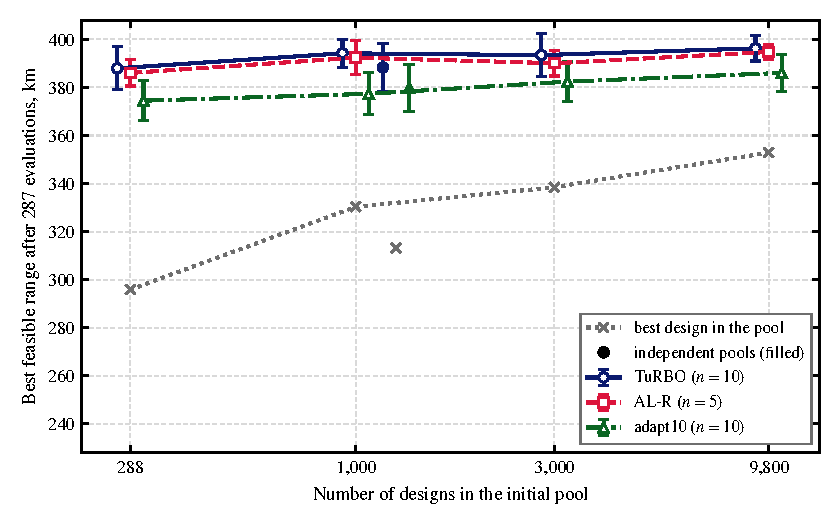
\includegraphics[width=0.8\linewidth]{figures/fig_pool_size.pdf}
\caption{Best feasible range after 287 evaluations as a function of the size of the initial pool (mean and standard deviation over seeds; the three strategies are offset horizontally for clarity). The dotted line is the mean best design in the pool before the search. Filled symbols at 1{,}000 designs are the runs from independent pools.}
\label{fig:pool_size}
\end{figure}

\textbf{A subsample one tenth the size of the pool costs the model-based strategies little.} From 1{,}000 pool designs TuRBO reaches \NpTurboBMean\,km, which is \NpTurboLossB\,km below its result from the full pool (Welch $p = \NpTurboLossBP$, bootstrap 95\% CI $\NpTurboLossBCI$\,km); from 3{,}000 designs the difference is \NpTurboLossC\,km ($p = \NpTurboLossCP$). Only the smallest pool costs a measurable amount: \NpTurboLossA\,km, or $\NpTurboLossAPct\%$ ($p = \NpTurboLossAP$). AL-R behaves in the same way on five seeds (\NpALRLossB\,km at 1{,}000 designs, $p = \NpALRLossBP$; \NpALRLossA\,km at 288, $p = \NpALRLossAP$). These non-significant differences are not evidence of equivalence, and the interval for TuRBO at 1{,}000 designs still allows a loss of several kilometers. They do show that most of the pool is not needed to reach the neighborhood of the best designs. This agrees with benchmark studies of unconstrained Bayesian optimization on test functions, which found small initial designs preferable~\cite{bossek2020initial,leriche2021revisiting}; the present result extends that observation to a constrained aircraft problem in which most of the sample is infeasible.

\textbf{A pool no larger than the search budget is enough to exceed the full pool.} With 288 initial designs and 287 further evaluations, \NpEvalsA\ in total, all \NpTurboABeatFull\ TuRBO runs and all \NpAdaptABeatFull\ adaptive-local runs end above the best of the 9{,}800 pool designs (\NpFullPoolBest\,km); the worst TuRBO run reaches \NpTurboAMin\,km. For comparison, the best design of a 288-design space-filling subsample averages \NpPoolABest\,km. Sequential search of any of the three kinds is therefore far more efficient than the space-filling sample on this problem, with about \NpEvalRatio\ times fewer evaluations for a longer range.

\textbf{The ordering of the strategies does not depend on the pool.} TuRBO is ahead of the adaptive local search at every pool size, by \NpTvAAD, \NpTvABD, \NpTvACD\ and \NpTvAFD\,km from the smallest pool to the full one ($p \le \NpTvAMaxP$ in each case), and TuRBO and AL-R are not distinguishable at any size on the five shared seeds ($p \ge \NpTvRMinP$). The surrogate-free search depends on the pool more than TuRBO does: it loses \NpAdaptLossB\,km at 1{,}000 designs ($p = \NpAdaptLossBP$) and \NpAdaptLossA\,km at 288 ($p = \NpAdaptLossAP$), because its parents are pool designs until better ones are found. The advantage of the model-based strategies over the surrogate-free control is therefore not produced by the large pool, and it is at least as large when the pool is small.

\textbf{Independent pools give a less favorable but consistent picture.} The subsamples above are drawn from the one pool and can inherit its best designs. As a check, ten fresh Latin hypercube pools of 1{,}000 designs were generated and evaluated, one for each seed, and TuRBO and the adaptive local search were run from them (last row of Table~\ref{tab:pool}, filled symbols in Fig.~\ref{fig:pool_size}). The best design of these pools averages \NpIndPoolBest\,km, against \NpPoolBBest\,km for the subsamples of the same size. TuRBO reaches $\NpIndTurboMean \pm \NpIndTurboSd$\,km, which is \NpIndTurboVsSubAbs\,km below its result on the subsamples (Welch $p = \NpIndTurboVsSubP$) and \NpIndTurboVsFull\,km below its result from the full pool ($p = \NpIndTurboVsFullP$); the adaptive local search reaches $\NpIndAdaptMean \pm \NpIndAdaptSd$\,km. TuRBO leads by \NpIndTvAD\,km (bootstrap 95\% CI $\NpIndTvACI$\,km, Welch $p = \NpIndTvAP$), the same direction as in every other row of the table but not significant at the 5\% level with ten runs. All \NpIndTurboBeatFull\ TuRBO runs and all \NpIndAdaptBeatFull\ adaptive-local runs again exceed the best of the full pool, with \NpIndEvals\ evaluations in total. Taken together, reducing the pool from 9{,}800 to 1{,}000 designs costs TuRBO between \NpTurboLossB\ and \NpIndTurboVsFull\,km ($\NpTurboLossBPct$ to $\NpIndTurboVsFullPct\%$), depending on whether the small pool happens to contain good designs. The means are also not monotone in the pool size (TuRBO at 3{,}000 against 1{,}000 designs), which shows the size of the seed-to-seed noise at ten runs.

\subsection{Role of the Classifier Weight and of the Washout Repair}
\label{sec:feas_ablation}
Table~\ref{tab:factorial} crosses the two ingredients of the active-learning acquisition that concern feasibility: the classifier weight $w(P_{\mathrm{feas}})$ (sigmoid, hard gate at $P_{\mathrm{feas}} \ge 0.5$, or absent) and the washout repair (sorting the four twist variables before evaluation). Each cell uses seeds 0 to 9.

\begin{table}[htbp]
\centering\small
\caption{Feasibility handling in the active-learning acquisition, ten seeds per row (TuRBO: 20, as in Table~\ref{tab:budget}), and the effect of adding the sigmoid weight to TuRBO (TuRBO+w). ``Sigmoid'', ``hard gate'' and ``none'' are the forms of the classifier weight and ``+R'' is the washout repair. Columns as in Table~\ref{tab:budget}.}
\label{tab:factorial}
\begin{tabular*}{\linewidth}{@{\extracolsep{\fill}}lrrrrrrrrr@{}}
\toprule
 & & \multicolumn{3}{c}{Best feasible range (km)} & \multicolumn{3}{c}{Share of evaluations (\%)} & \multicolumn{2}{c}{Beating the pool} \\
\cmidrule(lr){3-5}\cmidrule(lr){6-8}\cmidrule(l){9-10}
Strategy & Runs & at 100 & at 287 & min to max & valid & valid$_{60}$ & fail $g_8$ & runs & evals \\
\midrule
AL, sigmoid & 10 & 376.1 & 385.5 $\pm$ 10.8 & 368.9 to 397.4 & 60 & 14 & 17 & 10/10 & 44 \\
AL, sigmoid + R & 10 & 379.8 & 394.0 $\pm$ 4.1 & 386.3 to 399.5 & 65 & 26 & 0 & 10/10 & 32 \\
AL, none & 10 & n/a & none feasible & n/a & 0 & 0 & 100 & 0/10 & n/a \\
AL, none + R & 10 & n/a & none feasible & n/a & 0 & 0 & 0 & 0/10 & n/a \\
AL, hard gate & 10 & 352.9 & 394.0 $\pm$ 4.2 & 383.6 to 399.5 & 10 & 0 & 64 & 10/10 & 192 \\
TuRBO & 20 & 382.9 & 396.8 $\pm$ 4.4 & 385.3 to 403.0 & 82 & 80 & 0 & 20/20 & 2 \\
TuRBO+w & 10 & 383.9 & 397.5 $\pm$ 2.8 & 394.0 to 403.0 & 92 & 92 & 0 & 10/10 & 2 \\
\bottomrule
\end{tabular*}

\end{table}

\begin{figure}[htbp]
\centering
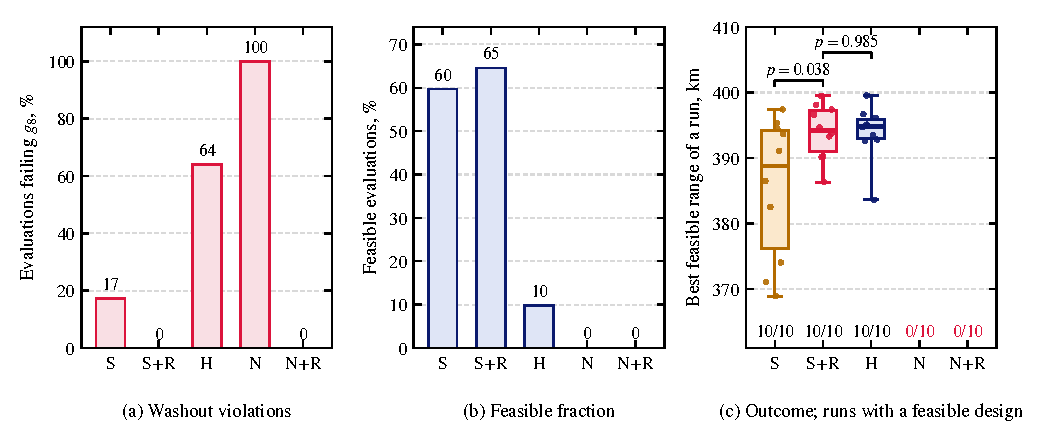
\includegraphics[width=\linewidth]{figures/fig_repair.pdf}
\caption{Feasibility handling in the active-learning loop (seeds 0 to 9). S: sigmoid weight; H: hard gate; N: no weight; +R: with the washout repair. (a) Share of evaluations that violate the washout ordering $g_8$ (\%; the repair makes it zero). (b) Share of feasible evaluations (\%). (c) Best feasible range of every run (dots) with quartiles, median and extremes; brackets give two-sided Welch $p$-values and the figures above the axis the number of runs that found a feasible design.}
\label{fig:repair}
\end{figure}

\textbf{Without a classifier weight the loop finds no feasible design.} This holds in all ten runs without the repair and in all ten runs with it. The regression surrogates are fitted on feasible designs only, so they carry no information about the constraint boundary, and the optimizer of the acquisition settles in a corner of the box (short center body, minimum blend chord, maximum battery mass) where the predicted range is high and the bay volume constraint $g_6$ is violated. The classifier is therefore a necessary component of this loop and not an optional refinement.

\textbf{The form of the weight is secondary.} A hard gate reaches $\NvMeanALhard \pm \NvSdALhard$\,km without the repair, against $\NvMeanALRten \pm \NvSdALRten$\,km for the sigmoid weight with the repair (no difference at the resolution of the table, Welch $p \NvPALhardvALRten$). The gate reaches this value late: only \NvValidALhard\% of its evaluations are feasible and its first improvement on the pool comes after a median of 192 evaluations, so its result at smaller budgets is worse than that of the sigmoid weight.

\textbf{The repair accounts for the gap between the published loop and AL-R.} With the sigmoid weight, sorting the twist variables raises the mean from $\NvMeanALrep \pm \NvSdALrep$ to $\NvMeanALRten \pm \NvSdALRten$\,km (\NvDALRtenvALrep\,km, Welch $p \NvPALRtenvALrep$, Mann--Whitney $p \NvUALRtenvALrep$, interval $\NvCIALRtenvALrep$\,km) and removes the low tail of the distribution (Fig.~\ref{fig:repair}). The evidence for this effect is moderate, not strong: the Mann--Whitney test does not reach the 5\% level, and with all available seeds the Holm-corrected value in Table~\ref{tab:tests} is $p \NvHALRvAL$.

\textbf{The weight does not help TuRBO.} Applying the same sigmoid weight to the Thompson samples of TuRBO changes the mean by $\NvDsTurboFeasFixvTurbo$\,km (Welch $p \NvPTurboFeasFixvTurbo$, bootstrap 95\% CI $\NvCITurboFeasFixvTurbo$\,km) while raising the feasible fraction from \NvValidTurbo\% to \NvValidTurboFeasFix\%. The same experiment with the first TuRBO implementation gave $\NvDsTurboFeasvTurboOld$\,km ($p \NvPTurboFeasvTurboOld$; Table~\ref{tab:asrun}), so neither version shows a gain in the mean. A trust region centered on a feasible design already keeps most candidates feasible, so the classifier adds little there. The weight is a requirement of a global acquisition built on feasible-only surrogates, not a general improvement to constrained search.

\subsection{Surrogate Distribution Shift and Extrapolation Performance}
\label{sec:distribution_shift}
The loop samples where the surrogate predicts high range, so the designs it proposes are not distributed like the pool on which the surrogate was trained. Two tests quantify the effect on the ensemble: (i) training on the pool and testing on the 157 feasible designs proposed by the original campaign, and (ii) a deliberately harsh extrapolation test, training on designs with $R < 250\,\mathrm{km}$ and testing on those with $R \ge 250\,\mathrm{km}$.

Table~\ref{tab:shift} and Fig.~\ref{fig:surrogate_parity} show a clear loss of accuracy. On the designs proposed by the loop the coefficient of determination for range falls from $0.997$ in cross-validation to $R^2 = \NshiftRtwo$, with a mean absolute error of $\NshiftMae\,\mathrm{km}$ that is almost entirely a bias ($\NshiftBias\,\mathrm{km}$): the ensemble underpredicts the range of the best designs. The rank correlation over all test designs remains high ($\rho = 0.95$), and $78\%$ of the test points lie within one ensemble standard deviation. Within the best tenth of the test designs, however, the rank correlation for range is close to zero ($\rho = -0.05$; $-0.02$ in the extrapolation test), and in the extrapolation test $R^2$ falls to $0.35$. The ensemble thus separates good designs from poor ones but does not order the best designs among themselves. This is consistent with the benchmark result that a search guided by this ensemble gains little over a local search that uses no surrogate (Section~\ref{sec:budget_results}).

\subsection{Cross-Solver Consistency with AeroBuildup}
\label{sec:aerobuildup_consistency}
\label{sec:validation}
To check that the ranking produced by the pipeline does not depend on its drag model, the pipeline was compared with AeroBuildup on $\NxN$ designs: the six best and six randomly chosen feasible designs of each of the first three seeds of the clamp and no-clamp searches of Section~\ref{sec:loft}, so that half of the sample comes from the top of the ranking. AeroBuildup is evaluated at the cruise lift coefficient of the pipeline.

As shown in Fig.~\ref{fig:aerobuildup_polar} and Fig.~\ref{fig:fidelity_suite}(a), the two solvers rank the designs alike: the Spearman correlation of $L/D$ is $\rho = \NxRho$ over the whole set and $\rho = \NxRhoTop$ among the 36 top designs. The absolute values differ considerably. AeroBuildup gives a higher $L/D$ than the pipeline on every design, with a median ratio of $\NxRatioMed$ (5th to 95th percentile $\NxRatioLo$ to $\NxRatioHi$). The difference comes mainly from profile drag: AeroBuildup uses NeuralFoil section polars with predicted transition, which give about two thirds of the pipeline's strip estimate (Supplementary Section~\ref{sec:neuralfoil_audit}). The pipeline is therefore pessimistic in absolute range relative to these models, and the absolute ranges in this paper should be read as estimates of a low-order model whose drag level has not been validated by experiment.

\paragraph{Panel refinement, section drag and Euler solutions} Three further checks are reported in the Supplementary Material and summarized in Fig.~\ref{fig:fidelity_suite}. Refining the lattice from 672 to 3{,}584 panels changes $L/D$ of the good designs by $0.6$ to $1.5\%$ and the static margin by less than $0.009$; only poor designs with closely spaced sections are sensitive to the finest grids, which become ill-conditioned (Supplementary Section~\ref{sec:grid_convergence}). NeuralFoil section polars give $0.60$ to $0.65$ times the strip estimate of profile drag with free transition and about $1.18$ times with forced transition, with little variation between designs, so the ranking is unaffected while the absolute range depends on how much laminar flow the airframe achieves (Supplementary Section~\ref{sec:neuralfoil_audit}). Euler solutions of five designs reproduce the lattice lift within $4\%$ for the three designs with a cruise $C_L$ above $0.2$, but give a static margin higher than the lattice value on every design, by a factor of $1.14$ to $1.28$; the best design of the original campaign has $SM = \NcfdChampSM$ in the Euler solution, above the $0.25$ limit (Supplementary Section~\ref{sec:cfd_validation}). Because the lattice underpredicts the margin, it is not conservative with respect to the upper limit, which motivates the calibration that follows.

\begin{figure*}[htbp]
\centering
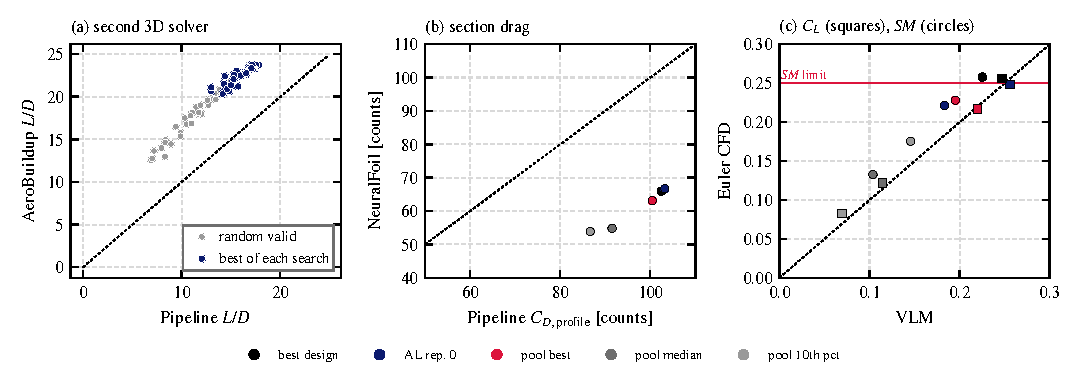
\includegraphics[width=\linewidth]{figures/fig_fidelity.pdf}
\caption{Multi-fidelity aerodynamic verification suite across computational tiers. (a) Cross-solver consistency between the baseline VLM pipeline and AeroBuildup across $n=72$ designs (Spearman $\rho = 0.98$ overall, $\rho = 0.91$ among the 36 top designs; median ratio $1.46$). (b) Viscous profile drag comparison between empirical strip theory and NeuralFoil ($e^N$ transition) across five representative configurations, with a ratio between $0.60$ and $0.65$. (c) 3D compressible Euler CFD using SU2 ($\sim 1.2 \times 10^5$ nodes) versus VLM predictions for lift coefficient $C_L$ (squares) and longitudinal static margin $SM$ (circles). The $C_L$ ratio lies between $0.97$ and $1.19$ and the Euler static margin is $1.14$ to $1.28$ times the lattice value. The best design of the original campaign reaches $SM = 0.258$ in the Euler solution, above the $0.25$ limit, whereas the best design of active-learning replication 0 has $SM = 0.221$.}
\label{fig:fidelity_suite}
\end{figure*}

\subsection{Calibrating the Static-Margin Constraint Against Euler CFD}
\label{sec:sm_calibration}
Five designs cannot define a correction for the static margin. The Euler analysis was therefore extended to \NcalNnew\ further designs, giving \NcalN\ in total: the best valid design of each of five search arms (TuRBO, active learning, adaptive local search, local search at $\pm 10\%$ and at $\pm 5\%$), and ten designs whose lattice margin lies near $0.05, 0.072, \ldots, 0.25$ (the valid design closest to each target among those with range at or above the pool median). Each case uses the setup of Supplementary Section~\ref{sec:cfd_validation} ($h = 7\,\mathrm{mm}$, $M = 0.11$, two angles of attack $2^\circ$ apart), and the Euler margin is $SM_{\mathrm{Euler}} = -\Delta C_{m}/\Delta C_{L}$ between them.

\begin{figure}[htbp]
\centering
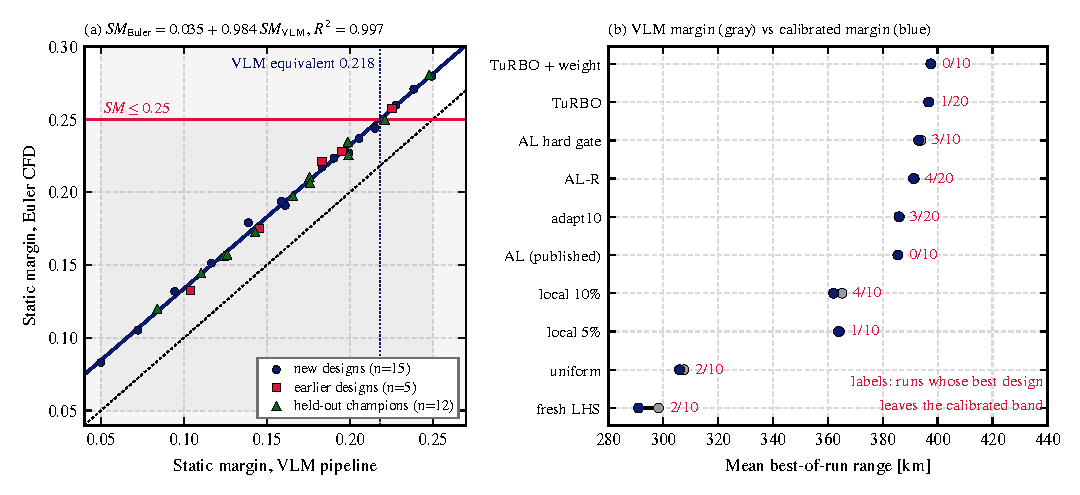
\includegraphics[width=\linewidth]{figures/fig_sm_calibration.pdf}
\caption{Calibration of the lattice static margin against Euler CFD. (a) Euler margin versus lattice margin for the \NcalN\ designs of the fit (circles and squares) with the least-squares line (blue), and for the \NoosN\ held-out run champions (triangles); the horizontal line is the $0.25$ cap and the dotted vertical line its lattice equivalent. (b) Mean best-of-run range of each search arm with the original lattice constraint (gray) and with the calibrated constraint applied after the fact (blue); the labels give the number of runs whose best design falls outside the calibrated band $0.05 \le SM \le 0.25$.}
\label{fig:sm_calibration}
\end{figure}

The relation is close to a constant shift (Fig.~\ref{fig:sm_calibration}a). A least-squares fit gives $SM_{\mathrm{Euler}} = \NcalA + \NcalB\,SM_{\mathrm{VLM}}$ with $R^2 = \NcalRsq$ and a residual standard deviation of \NcalSd; the 95\% bootstrap intervals are \NcalAci\ for the intercept and \NcalBci\ for the slope, so the slope is consistent with one and the offset with a constant of about \NcalA. The earlier ratio of $1.14\times$ to $1.28\times$ was therefore the same additive offset seen at different margins. The $C_L$ ratio between Euler and the lattice has a median of \NcalCLmed\ (range \NcalCLlo\ to \NcalCLhi) and does not show a trend. The offset moves the cap: $SM_{\mathrm{Euler}} \le 0.25$ corresponds to $SM_{\mathrm{VLM}} \le \NcalCapEquiv$, so a design that the optimizer treats as having a margin of $0.24$ has a margin near $0.27$ in Euler CFD. The lower cap of $0.05$ corresponds to a lattice value of \NcalFloorEquiv\ and is not active. A $5\,\mathrm{mm}$ surface mesh for the active-learning champion ($\NcalAlHfiveNodes\times 10^3$ nodes) changes its Euler margin from \NcalAlHsevenSM\ to \NcalAlHfiveSM\ ($\NcalAlHdelta\%$), far below the offset.

\paragraph{Out-of-sample check of the calibration} The fit above was made first and then frozen. Afterwards, Euler solutions were computed with the same setup for \NoosN\ further designs that played no part in it: the best design of six TuRBO runs, three AL-R runs and three adaptive-local runs of the corrected benchmark (Table~\ref{tab:oos}). Their lattice margins span \NoosVlmLo\ to \NoosVlmHi. The frozen line predicts the Euler margin of these designs with a root-mean-square error of \NoosRmse, a mean error of \NoosBias\ and a largest error of \NoosMax, which is the same size as the residual standard deviation of the fit (\NoosFitSd). The calibration therefore holds for the designs that the searches actually converge to, and not only for the designs it was fitted on. The check also bears on the cap. The calibration places \NoosPredOver\ of the \NoosN\ designs above $0.25$; the Euler solution confirms \NoosEulerOver\ (\NoosEulerHi) and puts the other at \NoosNearCap, which is on the cap to within the error of the fit. A decision closer to the cap than about \NoosMax\ therefore cannot be made from the calibrated lattice value alone.

\begin{table}[htbp]
\centering\small
\caption{Out-of-sample check of the static-margin calibration on \NoosN\ run champions that were not used in the fit. The prediction is $\NcalA + \NcalB\,SM_{\mathrm{VLM}}$ with the coefficients of Section~\ref{sec:sm_calibration} unchanged.}
\label{tab:oos}
% generated by b13_oos_validate.py; do not edit
\begin{tabular}{llrrrr}
\toprule
Strategy & Seed & Lattice $\mathrm{SM}$ & Predicted Euler $\mathrm{SM}$ & Euler $\mathrm{SM}$ & Error \\
\midrule
AL-R & 10 & 0.084 & 0.118 & 0.120 & $+0.002$ \\
TuRBO & 2 & 0.110 & 0.144 & 0.144 & $+0.000$ \\
TuRBO & 3 & 0.124 & 0.158 & 0.156 & $-0.001$ \\
TuRBO & 5 & 0.126 & 0.160 & 0.157 & $-0.002$ \\
AL-R & 11 & 0.143 & 0.176 & 0.173 & $-0.003$ \\
TuRBO & 0 & 0.166 & 0.198 & 0.198 & $-0.001$ \\
adapt10 & 12 & 0.176 & 0.208 & 0.210 & $+0.002$ \\
TuRBO & 4 & 0.176 & 0.209 & 0.206 & $-0.002$ \\
AL-R & 12 & 0.199 & 0.231 & 0.234 & $+0.004$ \\
adapt10 & 10 & 0.199 & 0.231 & 0.225 & $-0.006$ \\
TuRBO & 1 & 0.221 & 0.253 & 0.250 & $-0.003$ \\
adapt10 & 11 & 0.248 & 0.279 & 0.281 & $+0.001$ \\
\midrule
\multicolumn{5}{l}{Root-mean-square error} & 0.003 \\
\multicolumn{5}{l}{Largest absolute error} & 0.006 \\
\bottomrule
\end{tabular}

\end{table}

Table~\ref{tab:sm_rerank} applies the fitted correction after the fact to every run: the best-of-run range is recomputed over the designs that satisfy $0.05 \le a + b\,SM_{\mathrm{VLM}} \le 0.25$. No search was repeated, and only designs that the original run had accepted can be recovered, so the calibrated feasible set is a subset of the original one. The effect on the mean best range is small for the adaptive strategies, at most \NcalLossAlHard\,km, and the ranking of the arms does not change. What changes is feasibility. The best design lies outside the calibrated band in \NcalOutLocTen\ of \NcalOutNLocTen\ static local-search ($\pm 10\%$) runs, \NcalOutAlHard\ of \NcalOutNAlHard\ runs of active learning with a hard gate, \NcalOutAlR\ of \NcalOutNAlR\ AL-R runs, \NcalOutAdapt\ of \NcalOutNAdapt\ adaptive-local runs and \NcalOutTurbo\ of \NcalOutNTurbo\ TuRBO runs, and in none of the \NcalOutNAlSoft\ runs of the published loop. The effect is therefore not confined to one kind of strategy: any search that converges toward the upper limit of the margin can end slightly beyond the calibrated limit. In each such run another design within the band is almost as good, which is why the loss in range is small. This agrees with the CFD result for the original campaign champion ($SM_{\mathrm{Euler}} = 0.258$). Euler CFD is itself an inviscid model, so the calibration maps one low-order model onto a better one and does not establish the true margin; wind-tunnel or flight data would be needed for that.

\subsection{Range Cost of Each Bound}
\label{sec:bound_prices}
Section~\ref{sec:bound_sensitivity} shows that relaxing four bounds together raises the range, but not which bound matters. To measure that, TuRBO was rerun on the same pool and budget with exactly one bound widened by $10\%$ of that variable's range, five seeds per bound: the lower taper-ratio bound ($0.55 \to 0.525$), the upper winglet-twist bound ($0 \to +1^\circ$), the upper battery-mass bound ($3.5 \to 3.7\,\mathrm{kg}$), and the lower cruise-speed bound ($36.1 \to 33.6\,\mathrm{m/s}$). The speed bound is the $130\,\mathrm{km/h}$ mission requirement, so that run measures what the requirement costs, not an engineering limit. The lower bound of $c_{\mathrm{blend}}$ could not be tested because the geometry code clips $c_{\mathrm{blend}}$ to at least $0.25\,\mathrm{m}$ regardless of the bound. The reference is the same TuRBO implementation on the original bounds ($n = 10$, \NbpRefMean\,km $\pm$ \NbpRefSd\,km). These runs use the corrected TuRBO implementation; the same experiment with the first implementation is retained in the data archive and gave the same pattern, with a measurable price for the battery-mass bound only.

\begin{table}[htbp]
\centering\small
\caption{Range gained by widening a single bound by $10\%$ of its range (TuRBO, 287 evaluations after the pool, five seeds per bound), against TuRBO on the original bounds. The confidence interval is a bootstrap interval on the difference of means (20{,}000 resamples), and $p$ is a two-sided Welch test. The last column is the share of runs whose best design lies within $2\%$ of the variable's range of the new limit. The cruise-speed bound is the mission requirement.}
\label{tab:bound_prices}
\begin{tabular*}{\linewidth}{@{\extracolsep{\fill}}llrrrcrr@{}}
\toprule
 & & & & \multicolumn{3}{c}{Gain over the original bounds} & \\
\cmidrule(lr){5-7}
Bound & Change & Runs & Best (km) & km & 95\% CI (km) & Welch $p$ & At new bound \\
\midrule
None & original bounds & 10 & 396.3 $\pm$ 5.3 & n/a & n/a & n/a & n/a \\
Taper ratio, lower & $0.55 \to 0.525$ & 5 & 398.7 $\pm$ 7.3 & $+2.4$ & $[-4.5,\ 8.3]$ & 0.530 & 60\% \\
Winglet twist, upper & $0 \to +1^\circ$ & 5 & 395.7 $\pm$ 4.3 & $-0.6$ & $[-5.1,\ 4.0]$ & 0.831 & 0\% \\
Battery mass, upper & $3.5 \to 3.7$\,kg & 5 & 417.3 $\pm$ 3.0 & $+21.0$ & $[17.2,\ 25.0]$ & $<$0.001 & 100\% \\
Cruise speed, lower & $36.1 \to 33.6$\,m/s & 5 & 395.8 $\pm$ 3.5 & $-0.5$ & $[-4.5,\ 3.9]$ & 0.831 & 0\% \\
\bottomrule
\end{tabular*}

\end{table}

Only the battery-mass bound has a measurable price (Table~\ref{tab:bound_prices}, Fig.~\ref{fig:bound_robust}a): raising it by $0.2\,\mathrm{kg}$ gained \textbf{$\NbpBmassGain$\,km} ($+\NbpBmassGainPct\%$, bootstrap 95\% CI $\NbpBmassCI$\,km, $p \NbpBmassP$), and every run ended at the new limit. That is close to proportional, since the extra mass is \NbpBmassMassPct\% of the bound and the range gain is \NbpBmassGainPct\%, as expected when the energy carried sets the range. The other three bounds gave $\NbpTaperGain$\,km (taper, $p = \NbpTaperP$), $\NbpWtwistGain$\,km (winglet twist, $p = \NbpWtwistP$) and $\NbpSpeedGain$\,km (speed, $p = \NbpSpeedP$), each indistinguishable from zero with five runs; their confidence intervals ($\NbpTaperCI$, $\NbpWtwistCI$ and $\NbpSpeedCI$\,km) leave room for gains of a few kilometers, so small effects cannot be excluded. With the speed bound lowered, \NbpSpeedAtBound\% of the runs ended near the new limit, so the search did not use the extra room. The optimum is therefore limited mainly by how much energy the airframe may carry, and a search in the nominal box cannot trade that against the other variables.

\begin{figure}[htbp]
\centering
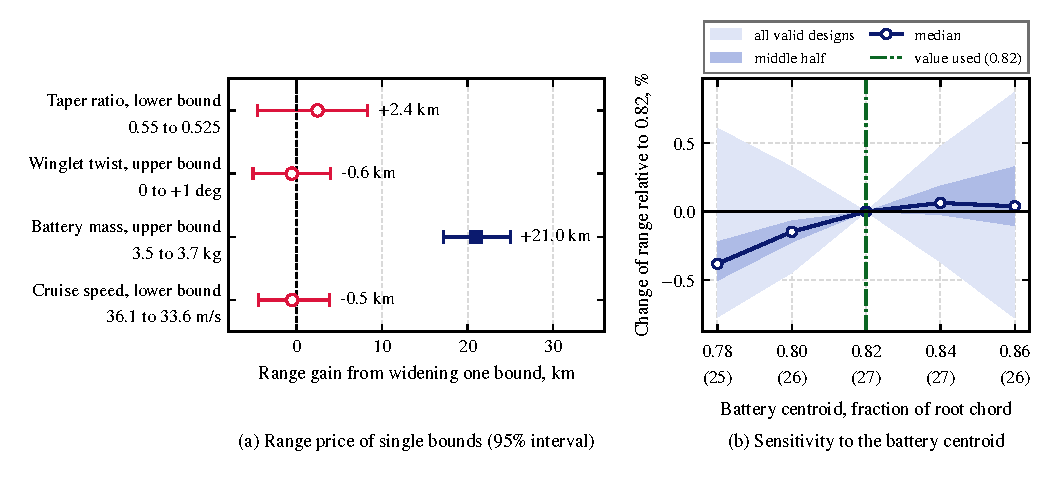
\includegraphics[width=\linewidth]{figures/fig_bound_robust.pdf}
\caption{(a) Range gained by widening each bound by 10\% of its range: difference of means against TuRBO on the original bounds with bootstrap 95\% intervals; the filled square is significant (Welch $p < 0.05$). (b) Change of calm-air range when the battery centroid is moved between 0.78 and 0.86 of the root chord, relative to the default 0.82, over the best designs of all search arms: median, middle half and full spread of the designs that remain valid, whose number is given in parentheses.}
\label{fig:bound_robust}
\end{figure}

\subsection{Robustness to the Battery Centroid and Battery Mass}
\label{sec:robustness}
The optimization fixes the battery centroid at $0.82\,c_{r}$ (Section~\ref{sec:dynamic_balance}). To check how much the conclusions depend on that value, \NrbN\ designs (the twenty best valid designs found by any arm, the best design of each arm and the original campaign champion, without duplicates) were reevaluated with the full pipeline at centroid positions from $0.78$ to $0.86\,c_{r}$ and with the battery mass changed by $\pm 5\%$. Moving the centroid by $\pm 0.04\,c_{r}$ changes the range by at most \NrbBandLossMax\% for any design that stays valid (Fig.~\ref{fig:bound_robust}b), and \NrbBandValid\ of the \NrbN\ designs stay valid over the whole interval. The best design that survives every perturbation is \NrbAllBest\ with \NrbAllBestRange\,km, which loses \NrbAllBestMfiveLoss\% of its range when the battery mass is reduced by $5\%$ and gains \NrbAllBestPfiveGain\% when it is increased; reducing the mass costs about \NrbMfiveLossMean\% of range on average, in line with the energy carried. The $+5\%$ case makes \NrbPfiveInvalid\ of the \NrbN\ designs invalid, and every one of these failures comes from the evaluator's check that rejects designs whose span efficiency factor exceeds one (values between $1.000$ and $1.006$). The best designs thus lie at the edge of a region the evaluator considers non-physical, which is a further active limit that is not among the box bounds and is consistent with reading the optima as boundary-limited. Only \NrbAllValid\ of the \NrbN\ designs are valid in all five centroid positions and both mass changes.

\subsection{Characteristics of the Audited Designs}
\label{sec:champion_characteristics}
Table~\ref{tab:best} lists the characteristics of the best design of the original campaign and of the best design of active-learning replication 0, the two designs for which Euler solutions and all audits are available. Neither is the best design found in the benchmark (Table~\ref{tab:budget}).

\paragraph{What the best designs of the benchmark have in common} Figure~\ref{fig:champions} shows the best design of each of the \NwinN\ runs of TuRBO, AL-R and the adaptive local search. Two variables are at a bound in nearly every run: the battery mass is within $3\%$ of its range from the upper bound in $\NwinBmassAt\%$ of the runs and the cruise speed within $3\%$ of the lower bound in $\NwinSpeedAt\%$. The blend chord and the taper ratio are at their lower bounds in $\NwinCblendAt\%$ and $\NwinTaperAt\%$ of the runs. The other ten variables are not determined by the search: across runs their standard deviation is $\NwinFreeSdLo\%$ to $\NwinFreeSdHi\%$ of the allowed range. The \NwinTopN\ runs that end within \NwinTopBand\,km of the best run have $L/D$ between \NwinTopLDlo\ and \NwinTopLDhi\ with inner sweeps from $\NwinTopSwInLo^\circ$ to $\NwinTopSwInHi^\circ$, outer sweeps from $\NwinTopSwOutLo^\circ$ to $\NwinTopSwOutHi^\circ$ and lattice static margins from \NwinTopSMlo\ to \NwinTopSMhi. The range is therefore set by the energy carried, the cruise speed and a small wing area, and it is nearly flat in sweep, twist distribution and winglet geometry at this fidelity. The strategies also settle in different parts of this flat region: the best TuRBO designs have a longer root chord and a blend station further inboard than the best AL-R designs (mean $c_r$ of \NwinTurboCr\ against \NwinAlrCr\,m and mean $y_b$ of \NwinTurboYb\ against \NwinAlrYb\,m, Mann--Whitney $p \NwinCrP$ and $p \NwinYbP$), at ranges that differ by about one percent. A conceptual study of this kind can thus report the active bounds and the attainable range with some confidence, but it does not identify a unique planform.

\begin{figure}[htbp]
\centering
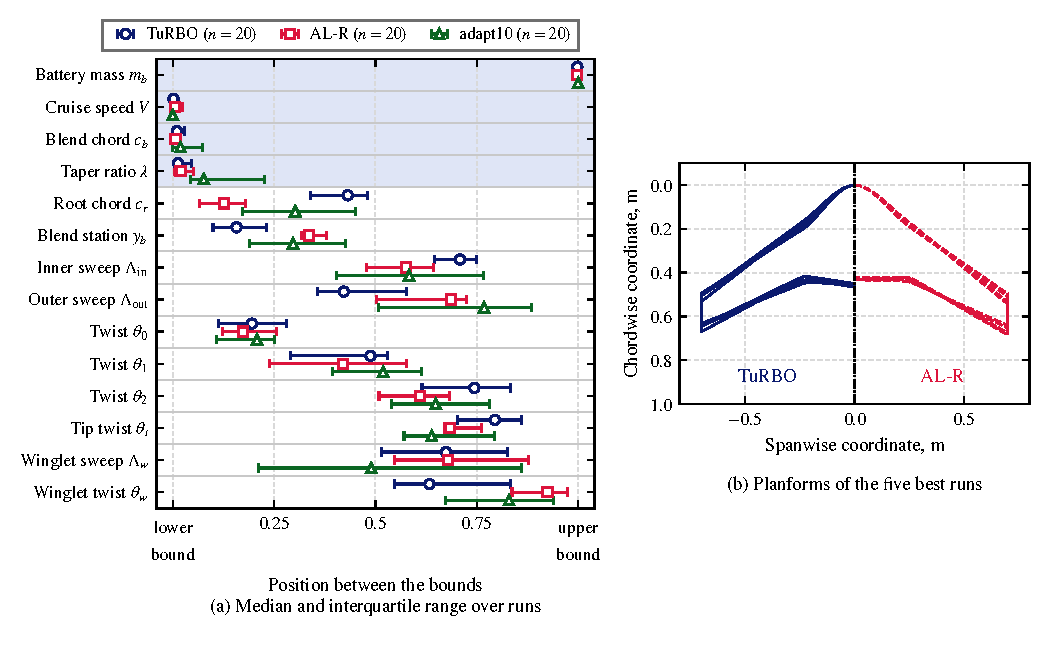
\includegraphics[width=\linewidth]{figures/fig_champions.pdf}
\caption{Best design of every run of TuRBO, AL-R and the adaptive local search. (a) Position of each design variable between its bounds: median and interquartile range over the runs of each strategy; the four shaded variables are those that end at a bound. (b) Planforms, without winglets, of the five best TuRBO runs (left, solid) and the five best AL-R runs (right, dashed).}
\label{fig:champions}
\end{figure}

The best design of the original campaign has an aspect ratio of $\NchAR$ and a reference area of $S_{\mathrm{ref}} = \NchSref\,\mathrm{m^2}$. At a cruise speed of $V = \NchV\,\mathrm{m/s}$ ($\NchVkmh\,\mathrm{km/h}$) the pipeline gives $L/D = \NchLD$, a calm-air range of $R = \NchampRange\,\mathrm{km}$, a lattice static margin of $SM = \NchSMpct\%$ and a cruise pitching moment of $C_m = \NchCm$. Its center of gravity lies at $42\%$ of the mean aerodynamic chord, slightly aft of the $15$ to $40\%$ window that the evaluator penalizes softly. The best designs of the benchmark runs differ from it mainly in using almost the full battery-mass allowance ($3.45$ to $3.50\,\mathrm{kg}$) close to the lowest permitted cruise speed.

\section{Discussion and Engineering Implications}
\label{sec:discussion}

\subsection{What the Benchmark Says About Surrogate-Assisted Search}
\label{sec:boundary_dominance}
The benchmark separates three sources of gain over the pool best. The first is local exploitation: perturbing the 20 best pool designs raises the best range from \NvPool\ to \NvMeanLocTen\,km. The second is letting the search center move, which adds \NvDAdaptvLocTen\,km without any model. The third is the model. For the active-learning loop as originally implemented it adds nothing measurable over the adaptive local search ($\NvDsALvAdapt$\,km, interval $\NvCIALvAdapt$\,km); with the washout repair it adds \NvDALRvAdapt\,km; for TuRBO it adds \NvDTurbovAdapt\,km. A claim that a surrogate-assisted loop outperforms its initial sample therefore says little: here \NvShareAdapt\% of the gain of the best strategy is available without a surrogate.

Three practical points follow. The first concerns the initial sample. The pool of 9{,}800 designs took $97\%$ of the evaluations, yet TuRBO started from 1{,}000 designs ends \NpTurboLossB\ to \NpIndTurboVsFull\,km below its full-pool result, and from 288 of them it still exceeds the best pool design in every run (Section~\ref{sec:pool_size}). For a model-based search on this problem a pool a few times the search budget recovers all but about $\NpIndTurboVsFullPct\%$ of the range, and evaluations beyond that are better spent on the search. The other two concern the strategies themselves. A constraint that can be satisfied by construction should be repaired before evaluation in every strategy; leaving it to a classifier cost the published loop \NvWashAL\% of its budget and most of its advantage. And a local Gaussian-process model with a trust region was both simpler to run and more reliable than a global neural ensemble with a classifier: it produced no exhausted run, the highest feasible fraction, and the best mean. The global loop remains useful where a feasibility model is wanted for other purposes, and its result after repair is \NvPctTurbovALR\% below that of TuRBO, but the data do not favor it for this problem.

\subsection{Bounds, Constraint Fidelity and the Search Strategy}
\label{sec:decoupling_contributions}
Relaxing four bounds together raised the mean best range of a simple elite search from \NpaperBndMean\ to \NwideBndMean\,km (Section~\ref{sec:bound_sensitivity}), several times the spread between the three leading strategies in Table~\ref{tab:budget}. The single-bound runs attribute this mainly to battery mass: $0.2$\,kg more battery gives \NbpBmassGain\,km, more than the difference between TuRBO and the adaptive local search. Suo et al.\ report the analogous result for a fuel-powered BWB UAV, where the fuel mass dominates the sensitivity of range~\cite{suo2026kriging}. The best designs sit at the battery-mass limit and close to the lowest permitted cruise speed, so the result of any strategy is set largely by those two requirements, and none of the designs should be described as a global optimum of the vehicle.

The fidelity of the stability constraint matters in a different way. The Euler calibration does not change the ranking of the strategies, but it moves the effective upper limit on the lattice margin from $0.25$ to \NcalCapEquiv, and the best design of \NcalOutLocTen\ of \NcalOutNLocTen\ static-local runs, \NcalOutAlR\ of \NcalOutNAlR\ AL-R runs, \NcalOutAdapt\ of \NcalOutNAdapt\ adaptive-local runs and \NcalOutTurbo\ of \NcalOutNTurbo\ TuRBO runs falls outside the calibrated band. A search that pushes against a constraint evaluated by a low-order model will find the model's error, and the calibrated limit should be used in the constraint from the start in future work.

The chord clamp of the loft is a validity guard. Inside the working bounds it is never active, and with widened bounds a search with the clamp and one without it reach the same range within the uncertainty of ten paired seeds. The loft does not make the center-body chord monotone (Section~\ref{sec:loft_def}); the excursions are below six millimeters and have no aerodynamic significance at this fidelity, but the earlier description of the loft as monotone by construction was incorrect.

\subsection{Limitations}
\label{sec:limitations}
\begin{itemize}
    \item \textbf{One aircraft, one pipeline, one budget.} All conclusions about search strategies hold for this 14-variable problem, this evaluator and 287 further evaluations. The ordering was checked for pools of 288 to 9{,}800 designs drawn from one Latin hypercube sample, for ten independent pools of 1{,}000 designs (Section~\ref{sec:pool_size}), and for budgets of 50 to 287 evaluations (Table~\ref{tab:anytime}); on the independent pools the lead of TuRBO over the adaptive local search has the same sign but does not reach the 5\% level. At twice the budget the ordering is unchanged and the gaps are smaller (Table~\ref{tab:long}). A more expensive evaluator, which would allow fewer evaluations, could change the ordering, and a recent benchmark of aerodynamic shape optimizers over 103 tasks found that optimizer rankings vary substantially between problem classes~\cite{fazliani2026shapebench}, so the ordering found here should not be assumed for other aircraft problems.
    \item \textbf{No viscous three-dimensional validation and no experiment.} The lattice assumes attached inviscid flow; at the cruise condition of the best designs ($C_L \approx 0.25$, $\alpha \approx 4^\circ$ in the lattice) this is plausible but unverified. Profile drag is a strip estimate with an assumed transition location, and AeroBuildup, whose section drag comes from NeuralFoil, gives an $L/D$ higher by a median factor of $1.46$. The Euler solutions check lift and the static margin only, on meshes that are not converged to better than about $5\%$ in lift, and contain no boundary layer. Absolute range and the true static margin require RANS solutions or wind-tunnel and flight data.
    \item \textbf{Stability constraint.} The optimization used the lattice static margin, which the Euler solutions show to be low by about $0.035$; the correction was confirmed on \NoosN\ designs outside the fit but only against Euler solutions. The calibrated constraint was applied after the fact and not inside a search. Lateral-directional stability, control power, aeroelastic effects and structural sizing are not modeled.
    \item \textbf{Mass and energy model.} The airframe mass is a linear function of reference area, the propulsive efficiency is an assumed four-point map, and the usable energy assumes $80\%$ depth of discharge at a steady $0.28\,C$ discharge. Range is linear in the usable energy, so these assumptions rescale all designs equally and do not affect the comparisons.
    \item \textbf{Fixed battery centroid and bay packaging.} The battery centroid is held at $0.82\,c_{r}$ for every design; it is never optimized and is not checked against the bay geometry. The packaging check integrates a center-body volume along the span with $45\%$ of the local chord as usable width and does not constrain where the battery lies along the chord, so a detailed internal layout may not realize the assumed position. Section~\ref{sec:robustness} shows that the best designs tolerate a shift of $\pm 0.04\,c_r$.
    \item \textbf{Guards inside the evaluator.} The best designs lie at the battery-mass bound and close to the evaluator's span-efficiency guard ($e \le 1$), which is a numerical safeguard and not a physical limit for a wing with winglets. The optima reported here are optima of this evaluator including its guards.
    \item \textbf{Benchmark implementation.} The active-learning loop and the baselines are single implementations with untuned hyperparameters. Trust-region methods that model the constraints themselves, such as SCBO~\cite{eriksson2021scbo} and FuRBO~\cite{ascia2025furbo}, were not tested; they need constraint values, and the strategies compared here see only whether a design is feasible. Two implementation issues that affected the comparison were found and corrected during this study (Section~\ref{sec:budget_protocol}); others may remain. The code and all run histories are released so that the comparison can be checked.
    \item \textbf{Statistics.} Ten to twenty runs per strategy detect differences of several kilometers; smaller differences between the leading strategies cannot be resolved, and the confidence intervals state what remains possible.
\end{itemize}

\section{Conclusions}
\label{sec:conclusion}

Eight search strategies were compared under an equal budget of 287 evaluations beyond a shared pool of 9,800 designs on the conceptual design of a 1.5\,m-span, 8\,kg electric tailless blended-wing-body UAV, and the evaluator and its stability constraint were audited against independent models. The conclusions are the following.

\begin{enumerate}
    \item \textbf{Search strategies.} TuRBO gave the longest range, $\NvMeanTurbo \pm \NvSdTurbo$\,km (\NvGainPctTurbo\% above the pool best). The neural-ensemble active-learning loop as originally implemented reached $\NvMeanAL \pm \NvSdAL$\,km and was not better than an adaptive local search without a surrogate ($\NvMeanAdapt \pm \NvSdAdapt$\,km, Welch $p \NvPALvAdapt$). With a repair that enforces the washout ordering before evaluation it reached $\NvMeanALR \pm \NvSdALR$\,km, \NvDALRvAdapt\,km above the adaptive local search (Holm $p \NvHALRvAdapt$) and \NvDTurbovALR\,km below TuRBO (Welch $p \NvPTurbovALR$, Holm $p \NvHTurbovALR$, interval $\NvCITurbovALR$\,km). Adaptive local search alone recovers \NvShareAdapt\% of the gain of TuRBO over the pool. The ordering of TuRBO, AL-R and the adaptive local search is the same from pools of 288, 1{,}000 and 3{,}000 designs; a pool of 1{,}000 designs costs TuRBO \NpTurboLossB\,km when it is a subsample of the full pool and \NpIndTurboVsFull\,km when it is generated independently, and with 288 pool designs every TuRBO run still exceeds the best of the full pool. At twice the budget the ordering is unchanged, but the lead of TuRBO over the adaptive local search falls from \NlTvAAD\ to \NlTvACD\,km.
    \item \textbf{Feasibility handling.} The classifier weight is necessary for the active-learning loop: without it no feasible design was found in 20 runs, with or without the repair. Its form matters little at the full budget, and adding it to TuRBO raised the feasible fraction but not the mean range. Constraints that can be satisfied by construction should be repaired in every strategy before a benchmark is interpreted.
    \item \textbf{Stability constraint.} Euler CFD on \NcalN\ designs shows that the lattice static margin is low by a nearly constant \NcalA\ ($R^2 = \NcalRsq$). The $0.25$ cap therefore corresponds to a lattice value of \NcalCapEquiv. On \NoosN\ further run champions that were not used in the fit, the calibration predicts the Euler margin with a root-mean-square error of \NoosRmse. Applying the calibrated constraint leaves the ranking of the strategies unchanged, but the best design of a minority of runs of most strategies, with and without a surrogate, lies beyond the calibrated limit.
    \item \textbf{Bounds and loft.} Among single-bound relaxations only the battery-mass limit has a measurable price (\NbpBmassGain\,km for $0.2$\,kg); the best designs are limited by the energy they may carry and by the minimum cruise speed. The chord clamp of the planform loft is a validity guard with no detectable effect on range, and the loft does not guarantee a monotone center-body chord.
    \item \textbf{Evaluator.} Panel refinement changes $L/D$ of the good designs by $0.6$ to $1.5\%$, and the ranking agrees with AeroBuildup ($\rho = 0.98$), but absolute drag differs between the models by a median factor of $1.46$ and no viscous three-dimensional solution or experiment is available. Ranges are therefore comparative.
\end{enumerate}

The audit of the code against the text changed the results: two baselines were corrected, an asymmetry between strategies was removed, and one geometric claim was withdrawn. The first implementations are retained beside the corrected ones. For studies of this kind the recommendation is to include a surrogate-free control with the same proposal structure as the surrogate loop, to report all seeds including failed runs, and to calibrate any constraint that the optimum presses against with a higher-fidelity model before the search.


\section*{CRediT Author Statement}
\textbf{Mudit Atrey:} Conceptualization, Methodology, Software, Formal analysis, Investigation, Data curation, Writing -- original draft, Writing -- review \& editing, Visualization.

\section*{Declaration of Competing Interest}
The author declares that he has no known competing financial interests or personal relationships that could have appeared to influence the work reported in this paper.

\section*{Funding}
This research did not receive any specific grant from funding agencies in the public, commercial, or not-for-profit sectors.

\section*{Data and Code Availability}
The complete run histories of all computational experiments are openly deposited at \url{https://doi.org/10.5281/zenodo.22893592}: for every evaluation of the original campaign, of each benchmark, ablation, pool-size, bound-price and loft run, and of the grid and battery-position audits, the full 14-variable design vector, the calm-air range, the feasibility flag, the lift-to-drag ratio, the static margin and the pitching moment. The deposit also contains the Euler CFD solution files and the Python scripts that generate every table, figure and numerical macro of this paper from those files. No design data are withheld. The released evaluator computes ranges with a usable energy density of $208.25\,\mathrm{Wh/kg}$, a value set before the battery-pack derivation of Supplementary Section~\ref{sec:battery_pack}; its ranges are converted to the basis of this paper by the factor $203.3/208.25$, and the stored database values by $203.3/160.0$. With that conversion, re-evaluating the stored design vector of the best design of the original campaign with the released code reproduces the stored range within five parts per million.

\section*{Declaration of generative AI and AI-assisted technologies in the manuscript preparation process}
During the preparation of this work the author used Claude (Anthropic) and Gemini (Google) in order to assist with the planning of the computational experiments, the writing and running of the analysis and plotting scripts, the checking of the manuscript against the code and the run files, the literature search, and the drafting and editing of the text. The author directed the work, approved each experiment and claim, and verified the results, including rerunning the scripts that generate every reported value. After using these tools, the author reviewed and edited the content as needed and takes full responsibility for the content of the published article.

\section*{Acknowledgments}
The author acknowledges the scientific computing and aerospace engineering communities for developing and maintaining the open-source frameworks utilized throughout this research, including AeroSandbox, NeuralFoil, SU2, Gmsh, and scikit-learn.

\bibliographystyle{elsarticle-num}
\bibliography{references}

\end{document}

